% memorder/memorder.tex

\QuickQuizChapter{chp:memorder:Memory Ordering}{Memory Ordering}
\OriginallyPublished{Chapter}{chp:memorder:Memory Ordering}{Linux Kernel Memory Barriers}{kernel.org}{Howells2009membartxt}
\OriginallyPublished{Chapter}{chp:memorder:Memory Ordering}{A formal kernel memory-ordering model}{Linux Weekly News}{JadeAlglave2017LWN-LKMM-1,JadeAlglave2017LWN-LKMM-2}
%
\Epigraph{The art of progress is to preserve order amid change and to preserve change amid order.}{\emph{Alfred North Whitehead}}

인과성과 순차적 순서는 상당히 직관적이며, 해커들은 일반인들에 비해 이런
개념들을 잘 이해하고 있는 경향을 띄는 경우가 많습니다.
이런 직관들은 순차적 코드와, 락킹과 RCU 같은 표준적 상호배타성 메커니즘을
사용하는 병렬 코드를 작성하고, 분석하고, 디버깅 하는데 매우 강력한 도구가 될 수
있습니다.
불행히도, 표준적 메커니즘을 사용하지 않는 코드에서는 이런 직관들이 깨어지게
되는데, 그런 중요한 예 하나는 이런 표준 메커니즘들을 구현하는 코드입니다.
이 챕터는 동기화 도구들과 다른 성능이 중요한 코드를 구현하기 충분할 만큼
메모리의 순서 규칙에 대해 여러분이 이해할 수 있도록 돕습니다.
\iffalse

Causality and sequencing are deeply intuitive, and hackers often
tend to have a much stronger grasp of these concepts than does
the general population.
These intuitions can be extremely powerful tools when writing, analyzing,
and debugging both sequential code and parallel code that makes
use of standard mutual-exclusion mechanisms, such as locking and
RCU.
Unfortunately, these intuitions break down completely in face of
code that fails to use standard mechanisms, one important example
of course being the code that implements these standard mechanisms.
This chapter will help you gain an understanding of memory ordering
sufficient to implement synchronization primitives and other
performance-critical code.
\fi

@@@ roadmap @@@

\section{Ordering: Why and How?}
\label{sec:memorder:Ordering: Why and How?}

메모리 순서규칙의 필요성은
Listing~\ref{lst:memorder:Memory Misordering: Store-Buffering Litmus Test}
(\path{C-SB+o-o+o-o.litmus})
에 보인,
사소해 보이기도 하는 리트머스 테스트로부터 얻을 수 있는데, 이 테스트에서는
\co{exists} 절이 절대 trigger 되지 않을 것을 보장한다 생각할 수
있습니다.\footnote{
	순수주의자들은 이 \co{exists} 절이 절대 \emph{만족}되지 않는다고
	표현하겠는데, 여기선 assertion 비유를 위해 ``trigger'' 라는 표현을
	사용하겠습니다.}
무엇보다도, \co{exists} 절 안에서 \nbco{0:r2=0} 가 성립된다면,\footnote{
	즉, Thread~\co{P0()} 의 로컬 변수 \co{r2} 의 인스턴스는 0 값을
	갖습니다.
	리트머스 테스트 명명법의 문서를 위해선
	Section~\ref{sec:formal:Anatomy of a Litmus Test} 을 참고하세요.}
우린 Thread~\co{P0()} 의 \co{x1} 로드가 Thread~\co{P1()} 의 \co{x1} 스토어보다
먼저 일어났어야만 한다고 희망하게 되며, 이는 곧 Thread~\co{P1()} 의 \co{x0} 의
로드가 Thread~\co{P0()} 의 \co{x0} 스토어보다 나중에 일어나서 \nbco{1:r2=2}
이어서 \co{exists} 절이 trigger 되지 않게 되길 바라게 됩니다.
이 예제는 대칭적이므로, 비슷한 이유로 \nbco{1:r2=0} 는 \nbco{0:r2=2} 를
보장하길 기대하게 됩니다.
불행히도, 메모리 배리어의 부재는 이런 희망들을 없애버립니다.
CPU 는 비교적 강한 순서 규칙을 갖는 x86 과 같은 시스템에서조차도
Thread~\co{P0()} 와 Thread~\co{P1()} 모두 순서를 바꿀 권한을 가지고 있습니다.
\iffalse

One motivation for memory ordering can be seen in the trivial-seeming
litmus test in
Listing~\ref{lst:memorder:Memory Misordering: Store-Buffering Litmus Test}
(\path{C-SB+o-o+o-o.litmus})
appears to guarantee that the \co{exists} clause never triggers.\footnote{
	Purists would instead say that the \co{exists} clause is
	never \emph{satisfied}, but we use ``trigger'' here by
	analogy with assertions.}
After all, if \nbco{0:r2=0} as shown in the \co{exists} clause,\footnote{
	That is, Thread~\co{P0()}'s instance of local variable \co{r2}
	equals zero.
	See Section~\ref{sec:formal:Anatomy of a Litmus Test}
	for documentation of litmus-test nomenclature.}
we might hope that Thread~\co{P0()}'s
load from~\co{x1} must have happened before Thread~\co{P1()}'s store to~\co{x1},
which might raise
further hopes that Thread~\co{P1()}'s load from~\co{x0} must happen after
Thread~\co{P0()}'s store to~\co{x0}, so that \nbco{1:r2=2},
thus not triggering the \co{exists} clause.
The example is symmetric, so similar reasoning might lead
us to hope that \nbco{1:r2=0} guarantees that \nbco{0:r2=2}.
Unfortunately, the lack of memory barriers dashes these hopes.
The CPU is within its rights to reorder
the statements within both Thread~\co{P0()} and Thread~\co{P1()},
even on relatively strongly ordered systems such as x86.
\fi

\begin{listing}[tbp]
{ \scriptsize
\begin{verbbox}[\LstLineNo]
C C-SB+o-o+o-o
{
}

P0(int *x0, int *x1)
{
  int r2;

  WRITE_ONCE(*x0, 2);
  r2 = READ_ONCE(*x1);
}


P1(int *x0, int *x1)
{
  int r2;

  WRITE_ONCE(*x1, 2);
  r2 = READ_ONCE(*x0);
}

exists (1:r2=0 /\ 0:r2=0)
\end{verbbox}
}
\centering
\theverbbox
\caption{Memory Misordering: Store-Buffering Litmus Test}
\label{lst:memorder:Memory Misordering: Store-Buffering Litmus Test}
\end{listing}

\QuickQuiz{}
	컴파일러도
	Listing~\ref{lst:memorder:Memory Misordering: Store-Buffering Litmus Test}
	의 Thread~\co{P0()} 와 Thread~\co{P1()} 의 메모리 액세스 순서를 바꿀 수
	있죠, 그렇죠?
	\iffalse

	The compiler can also reorder Thread~\co{P0()}'s and
	Thread~\co{P1()}'s memory accesses in
	Listing~\ref{lst:memorder:Memory Misordering: Store-Buffering Litmus Test},
	right?
	\fi
\QuickQuizAnswer{
	일반적으로, 컴파일러 최적화는 CPU 가 할 수 있는 것보다 더 극단적이고
	심오한 순서 재배치를 가져옵니다.
	\co{READ_ONCE()} 와 \co{WRITE_ONCE()} 는 컴파일러가 순서를 재배치
	하는걸 막아줍니다.
	그리고 그외에도 많은 걸 막아주기 때문에, 이 섹션에서의 예제들은
	\co{READ_ONCE()} 와 \co{WRITE_ONCE()} 를 많이 사용할 겁니다.
	\iffalse

	In general, compiler optimizations carry out more extensive
	and profound reorderings than CPUs can.
	However, in this case, the volatile accesses in
	\co{READ_ONCE()} and \co{WRITE_ONCE()}
	prevent the compiler from reordering.
	And from doing much else as well, so the examples in this
	section will be making heavy use of
	\co{READ_ONCE()} and \co{WRITE_ONCE()}.
	% @@@ forward reference to a section describing READ_ONCE()
	% @@@ and WRITE_ONCE().
	\fi
} \QuickQuizEnd

이런 재배치에 대한 의지는
\co{litmus7}~\cite{Alglave:2014:HCM:2594291.2594347} 같은 도구를 통해 확인될 수
있는데, 이 도구는 제 x86 랩탑에서 100,000,000 번의 시도에서 314회 반직관적인
순서가 발생함을 찾아냈습니다.
이상하게 들리겠지만, 두 로드가 모두 값 2 를 리턴하는 경우는 덜 빈번하게
발생했는데, 이 경우엔 167번만 발생했습니다.\footnote{
	이 결과는 실제 하드웨어 구성, 얼마나 시스템에 부하가 가해졌는지,
	그외에도 많은것들에 예민하게 달라질 수 있음을 알아두시기 바랍니다.}
여기서의 교훈은 분명합니다: 증가된 반직관성은 확률의 감소를 의미하지 않습니다!
\iffalse

This willingness to reorder can be confirmed using tools such as
\co{litmus7}~\cite{Alglave:2014:HCM:2594291.2594347},
which found that the counter-intuitive ordering happened
314 times out of 100,000,000 trials on my x86 laptop.
Oddly enough, the perfectly legal outcome where both loads return the
value 2 occurred less frequently, in this case, only 167 times.\footnote{
	Please note that results are sensitive to the exact hardware
	configuration,
	how heavily the system is loaded, and much else besides.}
The lesson here is clear: Increased counterintuitivity does not necessarily
imply decreased probability!
\fi
% Run on June 23, 2017:
% litmus7 -r 1000 -carch X86 C-SB+o-o+o-o.litmus
% Test C-SB+o-o+o-o Allowed
% Histogram (4 states)
% 314   *>0:r2=0; 1:r2=0;
% 49999625:>0:r2=2; 1:r2=0;
% 49999894:>0:r2=0; 1:r2=2;
% 167   :>0:r2=2; 1:r2=2;

다음 섹션들은 이 직관이 정확히 어디서 깨졌는지 보이며, 이어서 여러분이 이런
문제들을 피할 수 있게 도와주는 메모리 배리어의 정신적 모델을 제공합니다.
\iffalse

The following sections show exactly where this intuition breaks down,
and then puts forward a mental model of memory barriers that can help
you avoid these pitfalls.
\fi

Section~\ref{sec:memorder:Why Hardware Misordering?}
왜 하드웨어 가 메모리 액세스들의 순서를 잘못 잡는지에 대한 짧은 소개를
제공하고, 이어서
Section~\ref{sec:memorder:How to Force Ordering?}
에서는 어떻게 여러분이 악의 사악한 하드웨어의 순서를 잘못잡는 계획을 좌절시킬
수 있는지에 대해 마찬가지로 짧은 소개를 제공합니다.
\iffalse

Section~\ref{sec:memorder:Why Hardware Misordering?}
gives a brief overview of why hardware misorders memory accesses, and then
Section~\ref{sec:memorder:How to Force Ordering?}
gives an equally brief overview of how you can thwart evil hardware
misordering schemes.
\fi

\subsection{Why Hardware Misordering?}
\label{sec:memorder:Why Hardware Misordering?}

하지만 대체 왜 메모리 배리어가 필요한거죠?
CPU 는 스스로 순서를 기록하고 있을 수 없는 건가요?
일단 그게 바로 우리가 어떤 것들을 기록하고 있기 위해 컴퓨터를 갖는 이유이지
않던가요?
\iffalse

But why are memory barriers needed in the first place?
Can't CPUs keep track of ordering on their own?
Isn't that why we have computers in the first place, to keep track of things?
\fi

많은 사람들이 실제로 자신의 컴퓨터가 사물에 대해 기록을 가지고 있을 것이라
기대합니다만, 많은 사람들은 또한 그 기록을 빠르게 관리할 것을 요구합니다.
하지만, Chapter~\ref{chp:Hardware and its Habits} 에서 보였듯이, 근래의 컴퓨터
시스템 제조사들이 직면한 어려움 중 한가지는 메인 메모리가 CPU 의 속도 향상을
따라가지 못한다는 것입니다---근래의 CPU 들은 메모리로부터 변수 하나의 값을
읽어오는데 필요한 시간 동안 수백개의 명령어를 실행할 수 있습니다.
따라서 CPU 들은
Figure~\ref{fig:cpu:System Hardware Architecture} 에서 보인 것과 같이
갈수록 커다란 캐시들을 갖추는데, 이는 특정 CPU 의 특정 변수로부터의 첫번째
로드가
Section~\ref{sec:cpu:Cache Misses} 에서 이야기한 값비싼 \emph{캐시 미스} 를
낸다 하더라도, 최초의 캐시 미스는 해당 변수가 해당 CPU 의 캐시에 올라오게 하기
때문에 해당 CPU 로부터 해당 변수로의 뒤이은 반복된 로드들은 매우 빠르게
수행됨을 의미합니다.
\iffalse

Many people do indeed expect their computers to keep track of things,
but many also insist that they keep track of things quickly.
However, as seen in Chapter~\ref{chp:Hardware and its Habits},
one difficulty that modern computer-system vendors face is that
the main memory cannot keep up with the CPU---modern CPUs can execute
hundreds of instructions in the time required to fetch a single variable
from memory.
CPUs therefore sport increasingly large caches, as seen back in
Figure~\ref{fig:cpu:System Hardware Architecture}, which means that
although the first load by a given CPU from a given variable will
result in an expensive \emph{cache miss} as was discussed in
Section~\ref{sec:cpu:Cache Misses}, subsequent
repeated loads from that variable by that CPU can execute
very quickly because the initial cache miss will have loaded that
variable into that CPU's cache.
\fi

하지만, 여러 CPU 들로부터 공유된 변수들 집합으로 이루어지는 빈번한 동시적
스토어들을 잘 처리할 필요 또한 있습니다.
Cache-coherent 시스템에서, 캐시들이 특정 변수의 여러 복사본들을 가지고 있다면,
이 모든 복사본들은 같은 값을 가져야만 합니다.
이는 동시의 읽기들에 대해서는 매우 잘 동작하지만, 동시의 쓰기들에 대해서는
그렇지 못합니다:  각각의 쓰기는 기존 값의 복사본들 모두에 대해서 어떤 일을
해줘야 하는데 (또다른 캐시 미스!), 이는 빛의 제한된 속도와 원자적 물질의 원리를
놓고 보면, 성급한 소프트웨어 해커들이 좋아하지 않을 만큼 느릴 겁니다.
\iffalse

However, it is also necessary to accommodate frequent concurrent stores
from multiple CPUs to a set of shared variables.
In cache-coherent systems, if the caches hold multiple copies of a given
variable, all the copies of that variable must have the same value.
This works extremely well for concurrent reads, but not so well for
concurrent writes:  Each write must do something about all
copies of the old value (another cache miss!), which, given the finite
speed of light and the atomic nature of matter, will be slower
than impatient software hackers would like.
\fi

\begin{figure}[tb]
\centering
\resizebox{2.5in}{!}{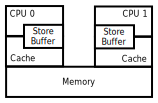
\includegraphics{memorder/SystemArchSB}}
\caption{System Architecture With Store Buffers}
\label{fig:memorder:System Architecture With Store Buffers}
\end{figure}

따라서 CPU 들은
Figure~\ref{fig:memorder:System Architecture With Store Buffers} 에 보인 것처럼
스토어 버퍼를 장착합니다.
특정 CPU 가 특정 변수에 스토어를 수행하는데 해당 변수가 해당 CPU 의 캐시에
존재하지 않는다면, 이 새로운 값은 해당 CPU 의 스토어 버퍼에 저장됩니다.
이 CPU 는 이제 이 스토어가 다른 CPU 들의 캐시들에 있을 수 있는 이 변수의 기존
값에 뭔가 작업을 수행할동안 기다리지 않고 곧바로 작업을 진행할 수 있습니다.
\iffalse

CPUs therefore come equipped with store buffers, as shown in
Figure~\ref{fig:memorder:System Architecture With Store Buffers}.
When a given CPU does a store to a given variable when that
variable is not present in that CPU's cache, then the new value
is instead placed in that CPU's store buffer.
The CPU can then proceed immediately, without having to wait for the
store to do something about all the old values of that variable
residing in other CPUs' caches.
\fi

\begin{figure}[htb]
\centering
\resizebox{3in}{!}{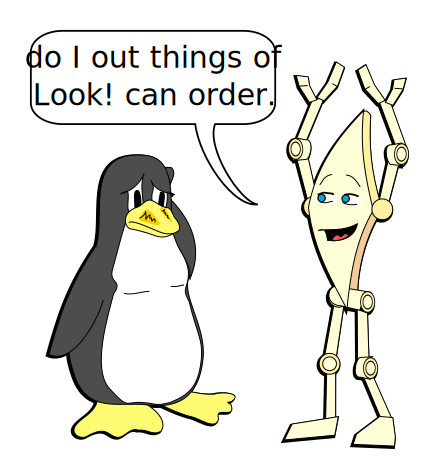
\includegraphics{cartoons/r-2014-Out-of-order}}
\caption{CPUs Can Do Things Out of Order}
\ContributedBy{Figure}{fig:memorder:CPUs Can Do Things Out of Order}{Melissa Broussard}
\end{figure}

스토어 버퍼들이 성능을 상당히 향상시킬 수 있지만, 이것들은 인스트럭션들과
메모리 참조들이 비순차적으로 수행되게 만들 수 있는데, 이는 곧 심각한 혼란을
가져오게 되는데, 이 상황이
Figure~\ref{fig:memorder:CPUs Can Do Things Out of Order} 에 그려져 있습니다.
구체적으로는, 이런 스토어 버퍼들이
Listing~\ref{lst:memorder:Memory Misordering: Store-Buffering Litmus Test} 에
보인 스토어 버퍼 리트머스 테스트에 보인 잘못된 메모리 순서를 가능하게 할 수
있습니다.
\iffalse

Although store buffers can greatly increase performance,
they can cause instructions and memory references to execute out
of order, which can in turn cause serious confusion, as illustrated in
Figure~\ref{fig:memorder:CPUs Can Do Things Out of Order}.
In particular, these store buffers can cause the memory misordering
shown in the store-buffering litmus test in
Listing~\ref{lst:memorder:Memory Misordering: Store-Buffering Litmus Test}.
\fi

\begin{table*}
\small
\centering\OneColumnHSpace{-0.1in}
\begin{tabular}{r||l|l|l||l|l|l}
	& \multicolumn{3}{c||}{CPU 0} & \multicolumn{3}{c}{CPU 1} \\
	\cline{2-7}
	& Instruction & Store Buffer & Cache &
		Instruction & Store Buffer & Cache \\
	\hline
	\hline
	1 & (Initial state) & & \tco{x1==0} &
		(Initial state) & & \tco{x0==0} \\
	\hline
	2 & \tco{x0 = 2;} & \tco{x0==2} & \tco{x1==0} &
		\tco{x1 = 2;} & \tco{x1==2} & \tco{x0==0} \\
	\hline
	3 & \tco{r2 = x1;} (0) & \tco{x0==2} & \tco{x1==0} &
		\tco{r2 = x0;} (0) & \tco{x1==2} & \tco{x0==0} \\
	\hline
	4 & (Read-invalidate) & \tco{x0==2} & \tco{x0==0} &
		(Read-invalidate) & \tco{x1==2} & \tco{x1==0} \\
	\hline
	5 & (Finish store) & & \tco{x0==2} &
		(Finish store) & & \tco{x1==2} \\
\end{tabular}
\caption{Memory Misordering: Store-Buffering Sequence of Events}
\label{tab:memorder:Memory Misordering: Store-Buffering Sequence of Events}
\end{table*}

Table~\ref{tab:memorder:Memory Misordering: Store-Buffering Sequence of Events}
은 이런 잘못된 메모리 접근 순서가 어떻게 일어날 수 있는지 보입니다.
Row~1 은 최초의 상태를 보이는데, 이 때 CPU~0 는 \co{x1} 을 자신의 캐시에 가지고
있고 CPU~1 은 \co{x0} 를 자기의 캐시에 가지고 있으며, 두 변수 모두 값 0을
가지고 있습니다.
Row~2 는 각 CPU 의 스토어 (
Listing~\ref{lst:memorder:Memory Misordering: Store-Buffering Litmus Test} 의
line~9 와~18) 로 인한 상태 변화를 보입니다.
두 CPU 모두 스토어가 향한 변수를 자신의 캐시에 가지고 있지 않았기에, 두 CPU 는
모두 각자의 스토어들을 자신의 스토어 버퍼들에서 처리합니다.
\iffalse

Table~\ref{tab:memorder:Memory Misordering: Store-Buffering Sequence of Events}
shows how this memory misordering can happen.
Row~1 shows the initial state, where CPU~0 has \co{x1} in its cache
and CPU~1 has \co{x0} in its cache, both variables having a value of zero.
Row~2 shows the state change due to each CPU's store (lines~9 and~18 of
Listing~\ref{lst:memorder:Memory Misordering: Store-Buffering Litmus Test}).
Because neither CPU has the stored-to variable in its cache, both CPUs
record their stores in their respective store buffers.
\fi

\QuickQuiz{}
	하지만 잠시만요!!!
	Table~\ref{tab:memorder:Memory Misordering: Store-Buffering Sequence of Events}
	의 row~2 에서 \co{x0} 와 \co{x1} 모두 동시에 두개의 값, 0 과 1 을
	가지고 있어요.
	어떻게 이게 가능한거죠???
	\iffalse

	But wait!!!
	On row~2 of
	Table~\ref{tab:memorder:Memory Misordering: Store-Buffering Sequence of Events}
	both \co{x0} and \co{x1} each have two values at the same time,
	namely zero and two.
	How can that possibly work???
	\fi
\QuickQuizAnswer{
	나중에 이야기 하겠지만, 아래쪽에 좀 더 일을 빠듯하게 처리되도록 하는
	cache-coherence 프로토콜이 존재합니다.
	하지만 어떤 변수가 동시에 두개의 값을 갖는다는게 신기하다고
	생각하신다면,
	Section~\ref{sec:memorder:Variables With Multiple Values} 까지
	잠깐 기다려 주시기 바랍니다.
	\iffalse

	There is an underlying cache-coherence protocol that straightens
	things out, which will be discussed later.
	% @@@ Add forward reference.
	But if you think that a given variable having two values at
	the same time is surprising, just wait until you get to
	Section~\ref{sec:memorder:Variables With Multiple Values}!
	\fi
} \QuickQuizEnd

Row~3 는 두개의 읽기
(Listing~\ref{lst:memorder:Memory Misordering: Store-Buffering Litmus Test} 의
line~10 과~19) 를 보입니다.
각 CPU 에 의해 읽혀지는 변수들은 각 CPU 의 캐시에 있기 때문에, 각각의 읽기는
곧바로 캐시의 값을 반환하는데, 이 경우 모두 0의 값입니다.

하지만 이 CPU 들은 일이 다 끝나지 않았습니다: 금방이든 나중이든, 각자의 스토어
버퍼를 비워야만 합니다.
캐시는 \emph{캐시라인 (cacheline)} 이라 불리는 상대적으로 커다란 블록 단위로
데이터를 옮기기 때문에, 그리고 각각의 캐시라인은 여러 변수들을 담고 있을 수
있기 때문에, 각 CPU 는 자신의 스토어 버퍼 안의 변수에 해당하는 캐시라인의 해당
변수에 해당하지 않는 부분은 만지지 않으면서 해당 변수에 해당하는 부분만을
업데이트 할 수 있도록 해당 캐시라인을 자신의 캐시로 가져와야만 합니다.
각 CPU 는 또한 해당 캐시라인이 어떤 다른 CPU 의 캐시에도 존재하지 않는다는 점을
보장해야만 하는데, 이를 위해 read-invalidate 오퍼레이션이 사용됩니다.
Row~4 에서 보인 것처럼, 두개의 read-invalidate 오퍼레이션이 완료된 후, 이 두
CPU 는 서로 넘겨받은 캐시라인들을 가지고 있게 되어서, CPU~0 의 캐시는 이제
\co{x0} 를 담고 있고 CPU~1 의 캐시는 \co{x1} 을 담고 있게 됩니다.
일단 이 두 변수들이 각자의 새로운 안식처에 위치하게 되면, 각 CPU 는 자신의
스토어 버퍼를 연관된 캐시 라인으로 비워낼 수 있게 되어서, 각 변수의 값을 row~5
에 보인 대로 마지막 값으로 설정합니다.
\iffalse

Row~3 shows the two reads (lines~10 and~19 of
Listing~\ref{lst:memorder:Memory Misordering: Store-Buffering Litmus Test}).
Because the variable being read by each CPU is in that CPU's cache,
each read immediately returns the cached value, which in both cases
is zero.

But the CPUs are not done yet: Sooner or later, they must empty their
store buffers.
Because caches move data around in relatively large blocks called
\emph{cachelines}, and because each cacheline can hold several
variables, each CPU must get the cacheline into its own cache so
that it can update the portion of that cacheline corresponding
to the variable in its store buffer, but without disturbing any
other part of the cacheline.
Each CPU must also ensure that the cacheline is not present in any other
CPU's cache, for which a read-invalidate operation is used.
As shown on row~4, after both read-invalidate operations complete,
the two CPUs have traded cachelines, so that CPU~0's cache now contains
\co{x0} and CPU~1's cache now contains \co{x1}.
Once these two variables are in their new homes, each CPU can flush
its store buffer into the corresponding cache line, leaving each
variable with its final value as shown on row~5.
\fi

\QuickQuiz{}
	하지만 이 값들은 또다시 캐시에서 메인 메모리로 비워져야 하는거
	아닌가요?
	\iffalse

	But don't the values also need to be flushed from the cache
	to main memory?
	\fi
\QuickQuizAnswer{
	놀라울 수 있겠지만, 꼭 그럴 필요는 없습니다!
	어떤 시스템들에서는, 두개의 변수들이 빈번하게 사용된다면, 이 변수들은
	CPU 의 캐시들 사이에서 움직이게 되고 메인 메모리에는 위치하지 않게
	됩니다.
	\iffalse

	Perhaps surprisingly, not necessarily!
	On some systems,
	if the two variables are being used heavily, they might
	be bounced back and forth between the CPUs' caches and never
	land in main memory.
	\fi
} \QuickQuizEnd

요약하자면, 스토어 버퍼들은 CPUe 들이 스토어 명령을 효과적으로 처리할 수 있도록
하기 위해 필요합니다만, 이게 반 직관적인, 잘못된 메모리 접근 순서를 야기할 수
있습니다.

하지만 여러분의 알고리즘이 정말로 메모리 참조의 순서를 맞춰야 한다면 어떻게
해야할까요?
예를 들어, 여러분이 어떤 드라이버와 하나는 이 드라이버가 동작 중인지 여부를 말하고 (driver-running flag) 하나는 이 드라이버에 처리되기를 기다리는 중인 요청이 있는지 여부를 말하는 (request-pending flag) 한쌍의 플래그를 사용해 통신하고 있다고 생각해 봅시다.
요청을 보내는 쪽은 request-pending flag 의 bit 을 채우고, driver-running flag 의 bit 을 검사한 후, 비어있다면 드라이버를 깨웁니다.
드라이버가 자신이 아는 모든 대기중인 요청들을 처리했다면, 드라이버는 자신의 driver-running flag 의 bit 을 없애고, 다시 일을 시작해야 하는지 여부를 보기 위해 request-pending flag 를 체크해야 합니다.
이 매우 합리적인 접근법도 하드웨어가 여기서의 스토어들과 로드들을 순서대로 처리한다고 보장할 수 있는 방법이 없다면 제대로 동작하지 않을 겁니다.
이게 다음 섹션의 주제입니다.
\iffalse

In summary, store buffers are needed to allow CPUs to handle
store instructions efficiently, but they can result in
counter-intuitive memory misordering.

But what do you do if your algorithm really needs its memory
references to be ordered?
For example, suppose that you are communicating with a driver using
a pair of flags, one that says whether or not the driver is running
and the other that says whether there is a request pending for that
driver.
The requester needs to set the request-pending flag, then check
the driver-running flag, and if false, wake it up.
Once the driver has serviced all the pending requests that it knows about,
it needs to clear its driver-running flag, then check the request-pending
flag to see if it needs to restart.
This very reasonable approach cannot work unless there is some way
to make sure that the hardware processes the stores and loads in order.
This is the subject of the next section.
\fi

\subsection{How to Force Ordering?}
\label{sec:memorder:How to Force Ordering?}

\emph{메모리 배리어} (예를 들어, 리눅스 커널의 \co{smp_mb()}) 를 사용해 순서
규칙의 환상을 지키는데 필요한 표준적 동기화 도구들 (락킹과 RCU 같은) 과
컴파일러 지시어들이 존재합니다.
이런 메모리 배리어들은 ARM, POWER, Itanium, 그리고 Alpha 에서처럼 명시적
인스트럭션이 될 수 있고, x86 에서 종종 그런 것처럼 다른 인스트럭션들에 의해
내포될 수도 있습니다.
이런 표준적 동기화 도구들은 순서가 지켜진다는 환상을 지키기 때문에, 여러분이
가장 쉽게 적용할 수 있는 방법은 그냥 이 도구들을 사용해서, 이 섹션을 그만 읽는
겁니다.
\iffalse

It turns out that there are compiler directives and standard
synchronization primitives (such as locking and RCU)
that are responsible for maintaining the illusion of ordering through use of
\emph{memory barriers} (for example, \co{smp_mb()} in the Linux kernel).
These memory barriers can be explicit instructions, as they are on
ARM, POWER, Itanium, and Alpha, or they can be implied by other instructions,
as they often are on x86.
Since these standard synchronization primitives preserve the illusion of
ordering, your path of least resistance is to simply use these primitives,
thus allowing you to stop reading this section.
\fi

\begin{listing}[tbp]
{ \scriptsize
\begin{verbbox}[\LstLineNo]
C C-SB+o-mb-o+o-mb-o
{
}

P0(int *x0, int *x1)
{
  int r2;

  WRITE_ONCE(*x0, 2);
  smp_mb();
  r2 = READ_ONCE(*x1);
}


P1(int *x0, int *x1)
{
  int r2;

  WRITE_ONCE(*x1, 2);
  smp_mb();
  r2 = READ_ONCE(*x0);
}

exists (1:r2=0 /\ 0:r2=0)
\end{verbbox}
}
\centering
\theverbbox
\caption{Memory Ordering: Store-Buffering Litmus Test}
\label{lst:memorder:Memory Ordering: Store-Buffering Litmus Test}
\end{listing}

하지만, 여러분 스스로 그런 동기화 도구들을 구현해야 한다면, 또는 그런 메모리
순서 규칙과 메모리 배리어가 어떻게 동작하는지에 그저 흥미가 있는 거라면, 계속
읽어주세요!
이 여정에서의 첫번째 정류장은
Listing~\ref{lst:memorder:Memory Ordering: Store-Buffering Litmus Test}
(\path{C-SB+o-mb-o+o-mb-o.litmus}) 으로, \co{smp_mb()} 리눅스 커널 메모리
배리어가 \co{P0()} 와 \co{P1()} 의 스토어와 로드 사이에 위치했다는 점을
제외하고는
Listing~\ref{lst:memorder:Memory Misordering: Store-Buffering Litmus Test} 에
보인 것과 동일한 코드입니다.
이 지시어들은 제 x86 랩탑에서의 100,000,000 번의 시도에도 반 직관적인 결과가
일어나는 것을 막았습니다.
흥미롭게도, 이 지시어들로 인해 추가된 오버헤드는 두 로드가 모두 값 2 를
반환하는 경우가 800,000 번이 넘게 일어나게 만들었는데, 이는 이 지시어가 없는
Listing~\ref{lst:memorder:Memory Misordering: Store-Buffering Litmus Test} 의
코드에서는 167 번밖에 일어나지 않았던 것과 대조적입니다.
\iffalse

However, if you need to implement the synchronization primitives
themselves, or if you are simply interested in understanding how memory
ordering and memory barriers work, read on!
The first stop on the journey is
Listing~\ref{lst:memorder:Memory Ordering: Store-Buffering Litmus Test}
(\path{C-SB+o-mb-o+o-mb-o.litmus}),
which the \co{smp_mb()} Linux-kernel full memory barrier placed between
the store and load in both \co{P0()} and \co{P1()}, but is otherwise
identical to the code shown in
Listing~\ref{lst:memorder:Memory Misordering: Store-Buffering Litmus Test}.
% Test C-SB+o-mb-o+o-mb-o Allowed
% Histogram (3 states)
% 49553298:>0:r2=2; 1:r2=0;
% 49636449:>0:r2=0; 1:r2=2;
% 810253:>0:r2=2; 1:r2=2;
% No
These directives prevent the counter-intuitive outcome from happening
on 100,000,000 trials on my x86 laptop.
Interestingly enough, the added overhead due to these directives causes the
legal outcome where both loads return the value two to happen more
than 800,000 times, as opposed to only 167 times for the
directive-free code in
Listing~\ref{lst:memorder:Memory Misordering: Store-Buffering Litmus Test}.
\fi

\begin{table*}
\small
\centering\OneColumnHSpace{-0.1in}
\begin{tabular}{r||l|l|l||l|l|l}
	& \multicolumn{3}{c||}{CPU 0} & \multicolumn{3}{c}{CPU 1} \\
	\cline{2-7}
	& Instruction & Store Buffer & Cache &
		Instruction & Store Buffer & Cache \\
	\hline
	\hline
	1 & (Initial state) & & \tco{x1==0} &
		(Initial state) & & \tco{x0==0} \\
	\hline
	2 & \tco{x0 = 2;} & \tco{x0==2} & \tco{x1==0} &
		\tco{x1 = 2;} & \tco{x1==2} & \tco{x0==0} \\
	\hline
	3 & \tco{smp_mb();} & \tco{x0==2} & \tco{x1==0} &
		\tco{smp_mb();} & \tco{x1==2} & \tco{x0==0} \\
	\hline
	4 & (Read-invalidate) & \tco{x0==2} & \tco{x0==0} &
		(Read-invalidate) & \tco{x1==2} & \tco{x1==0} \\
	\hline
	5 & (Finish store) & & \tco{x0==2} &
		(Finish store) & & \tco{x1==2} \\
	\hline
	6 & \tco{r2 = x1;} (2) & & \tco{x1==2} &
		\tco{r2 = x0;} (2) & & \tco{x0==2} \\
\end{tabular}
\caption{Memory Ordering: Store-Buffering Sequence of Events}
\label{tab:memorder:Memory Ordering: Store-Buffering Sequence of Events}
\end{table*}

이 지시어들은
Table~\ref{tab:memorder:Memory Ordering: Store-Buffering Sequence of Events} 에
보인 것과 같이 순서규칙에 깊은 영향을 끼칩니다.
앞의 두 행은
Table~\ref{tab:memorder:Memory Misordering: Store-Buffering Sequence of Events}
에 보인 것과 같고 row~3 의 \co{smp_mb()} 인스트럭션들은 직접적으로 상태를
바꾸지 않지만, 이 인스트럭션들은 스토어들이 (row~4 와~5) 로드 (row~6) 전에
완료되도록 만들어서,
Table~\ref{tab:memorder:Memory Misordering: Store-Buffering Sequence of Events}
에서 보인 반 직관적인 결과가 나타나지 못하게 합니다.
변수 \co{x0} 와 \co{x1} 은 row~2 에서 여전히 두개의 값을 갖지만, 앞서
약속한대로, 이 지시어들은 최종적으로는 일을 더 깐깐하게 처리했습니다.
\iffalse

These directives have a profound effect on ordering, as can be seen in
Table~\ref{tab:memorder:Memory Ordering: Store-Buffering Sequence of Events}.
Although the first two rows are the same as in
Table~\ref{tab:memorder:Memory Misordering: Store-Buffering Sequence of Events}
and although the \co{smp_mb()} instructions on row~3
do not change state
in and of themselves, they do cause the stores to complete
(rows~4 and~5) before the
loads (row~6), which rules out the counter-intuitive outcome shown in
Table~\ref{tab:memorder:Memory Misordering: Store-Buffering Sequence of Events}.
Note that variables \co{x0} and \co{x1} each still have more than one
value on row~2, however, as promised earlier, the directives straighten
things out in the end.
\fi

\begin{table*}
\small
\centering\OneColumnHSpace{-0.7in}
\begin{tabular}{l||c||c|c|c|c||c|c|c|c|c|c}
	& & \multicolumn{4}{c||}{Prior Ordered Operation} &
		\multicolumn{6}{c}{Subsequent Ordered Operation} \\
	\cline{3-6} \cline{7-12}
	Operation Providing Ordering & C &
		Self & R & W & RMW & Self & R & W & DR & DW & RMW \\
	\hline
	\hline
	\tco{READ_ONCE()} &  &
		   Y &   &   &     &      &   &   &    &  Y &     \\
	\hline
	\tco{smp_read_barrier_depends()} &  &
		     & Y &   &     &      &   &   &  Y &  Y &     \\
	\hline
	Successful \tco{*_acquire()} &   &
		   R &   &   &     &      & Y & Y &  Y &  Y &   Y \\
	\hline
	Successful \tco{*_release()} & C &
		     & Y & Y &   Y &    W &   &   &    &    &     \\
	\hline
	\tco{smp_rmb()} &   &
		     & Y &   &   R &      & Y &   &  Y &    &   R \\
	\hline
	\tco{smp_wmb()} &   &
		     &   & Y &   W &      &   & Y &    &  Y &   W \\
	\hline
	\tco{smp_mb()} & CP &
		     & Y & Y &   Y &      & Y & Y &  Y &  Y &   Y \\
	\hline
	Successful Non-Relaxed Non-\tco{void} RMW & CP &
		   Y & Y & Y &   Y &    Y & Y & Y &  Y &  Y &   Y \\
	\hline
	\tco{smp_mb__before_atomic()} & CP &
		     & Y & Y &   Y &      & a & a & a  & a  &   Y \\
	\hline
	\tco{smp_mb__after_atomic()} & CP &
		     & a & a &   Y &      & Y & Y &  Y &  Y &     \\
	\multicolumn{12}{c}{~} \\
	\multicolumn{1}{r}{Key:} &
		\multicolumn{11}{l}{C: Ordering is cumulative} \\
	\multicolumn{1}{r}{} &
		\multicolumn{11}{l}{P: Ordering propagates} \\
	\multicolumn{1}{r}{} &
		\multicolumn{11}{l}{R: Read, or read portion of RMW} \\
	\multicolumn{1}{r}{} &
		\multicolumn{11}{l}{W: Write, or write portion of RMW} \\
	\multicolumn{1}{r}{} &
		\multicolumn{11}{l}{Y: Provides the specified ordering} \\
	\multicolumn{1}{r}{} &
		\multicolumn{11}{l}{a: Provides specified ordering given intervening RMW atomic operation} \\
	\multicolumn{1}{r}{} &
		\multicolumn{11}{l}{DR: Dependent read (address dependency)} \\
	\multicolumn{1}{r}{} &
		\multicolumn{11}{l}{DW: Dependent write (address, data, or control dependency)} \\
	\multicolumn{1}{r}{} &
		\multicolumn{11}{l}{RMW: Atomic read-modify-write operation} \\
\end{tabular}
\caption{Linux-Kernel Memory-Ordering Cheat Sheet}
\label{tab:memorder:Linux-Kernel Memory-Ordering Cheat Sheet}
\end{table*}

\co{smp_mb()} 가 상당히 강력한 순서 보장을 갖긴 하지만, 그 강력함은 높은
비용으로부터 나옵니다.
굉장히 많은 상황들이 저렴한 메모리 배리어 인스트럭션을 사용하는, 또는, 어떤
경우에 있어서는, 아예 메모리 배리어 인스트럭션을 사용하지 않는 훨씬 약한 순서
보장만으로도 처리될 수 있습니다.
Table~\ref{tab:memorder:Linux-Kernel Memory-Ordering Cheat Sheet}
은 리눅스 커널의 순서 보장 도구들과 그 보장사항들을 보이는 커닝 페이퍼를
보입니다.
각 열은 순서 보장을 제공할 수도, 하지 않을 수도 있는 도구들 또는 도구들의
카테고리에 연관되며, ``Prior Ordered Operation'' 과 ``Subsequent Ordered
Operation'' 으로 라벨링된 행들은 각 열의 도구에 의해 순서가 맞춰지는 (또는
맞춰지지 않는) 오퍼레이션들입니다.
``Y'' 를 담는 셀들은 무조건적으로 순서가 제공됨을 의미하며, 다른 문자들은
순서가 부분적으로 또는 조건적으로 제공됨을 의미합니다.
빈 셀들은 어떤 순서 보장도 제공되지 않음을 의미합니다.
\iffalse

Although \co{smp_mb()} has extremely strong ordering guarantees, its strength
comes at a high price.
A great many situations can be handled with much weaker ordering guarantees
that use much cheaper memory-barrier instructions, or, in some case, no
memory-barrier instructions at all.
Table~\ref{tab:memorder:Linux-Kernel Memory-Ordering Cheat Sheet}
provides a cheatsheet of the Linux kernel's ordering primitives and their
guarantees.
Each row corresponds to a primitive or category of primitives that might
or might not provide ordering, with the columns labeled
``Prior Ordered Operation'' and ``Subsequent Ordered Operation''
being the operations that might (or might not) be ordered against.
Cells containing ``Y''indicate that ordering is supplied unconditionally,
while other characters indicate that ordering is supplied only partially or
conditionally.
Blank cells indicate that no ordering is supplied.
\fi

\co{*_acquire} 열은 \co{smp_load_acquire()}, \co{cmpxchg_acquire()},
\co{xchg_release()}, 등등을 포함합니다;
\co{*_release} 열은 \co{smp_store_release()}, \co{cmpxchg_release()},
\co{xchg_release()}, 등등을 포함합니다; 그리고
``Successful Non-Relaxed Non-\co{void} RMW'' 열은 \co{atomic_add_return()},
\co{atomic_add_unless()}, \co{atomic_dec_and_test()}, \co{cmpxchg()},
\co{xchg()}, 등등을 포함합니다.
``Successful'' 이라는 수식어는 실패했을 때에는 메모리에도 순서에도 어떤 영향을
끼치지 않는 \co{atomic_add_return()}, \co{cmpxchg_acquire()}, 그리고
\co{cmpxchg_release()} 같은 도구들에 적용됩니다.
\iffalse

The \co{*_acquire} row covers \co{smp_load_acquire()},
\co{cmpxchg_acquire()}, \co{xchg_release()}, and so on;
the \co{*_release} row covers \co{smp_store_release()},
\co{cmpxchg_release()}, \co{xchg_release()}, and so on; and
the ``Successful Non-Relaxed Non-\co{void} RMW'' row covers
\co{atomic_add_return()}, \co{atomic_add_unless()}, \co{atomic_dec_and_test()},
\co{cmpxchg()}, \co{xchg()}, and so on.
The ``Successful'' qualifiers apply to primitives such as
\co{atomic_add_unless()}, \co{cmpxchg_acquire()}, and \co{cmpxchg_release()},
which have no effect on either memory or on ordering when they indicate
failure.
\fi

``C'' 행은 누적성과 전파성을 의미하는데, 이에 대해서는
Sections~\ref{sec:memorder:Cumulativity}
과~\ref{sec:memorder:Propagation} 에서 설명됩니다.
해당 섹션을 읽기 전까지는, 이 행은 최대 두개 쓰레드만이 돌아가는 상황에서는
대부분 무시될 수 있다는 정도만 알아두면 되겠습니다.
\iffalse

Column ``C'' indicates cumulativity and propagation, as explained in
Sections~\ref{sec:memorder:Cumulativity}
and~\ref{sec:memorder:Propagation}.
In the meantime, this column can always be ignored when there
are at most two threads involved.
\fi

\QuickQuiz{}
	Table~\ref{tab:memorder:Linux-Kernel Memory-Ordering Cheat Sheet}
	의 열들은 상당히 무작위적이고 복잡해 보입니다.
	이 표의 개념적 근본이 무엇인가 있나요?
	\iffalse

	The rows in
	Table~\ref{tab:memorder:Linux-Kernel Memory-Ordering Cheat Sheet}
	seem quite random and confused.
	Whatever is the conceptual basis of this table???
	\fi
\QuickQuizAnswer{
	각 열들은 전력과 오버헤드가 증가되는 하드웨어 메커니즘들에 대략적으로
	연관되어 있습니다.

	\co{READ_ONCE()} 열은 (2017 년에 있어) 컴파일러들과 CPU 들은 사용자가
	볼 수 있는 예측적 스토어를 탐닉하지 않아서, 주소, 데이터, 또는 수행이
	앞의 로드에 의존적인 모든 쓰기는 해당 로드가 완료된 후에 행해진다는
	사실을 사용합니다.
	최소한 이런 의존성들이
	Sections~\ref{sec:memorder:Address- and Data-Dependency Restrictions}
	과~\ref{sec:memorder:Control-Dependency Restrictions} 에서 설명된 대로
	주의깊게 구성되었다는 가정 아래의 이야기입니다.
	\iffalse

	The rows correspond roughly to hardware mechanisms of increasing
	power and overhead.

	The \co{READ_ONCE()} row captures the fact that (as of 2017) compilers
	and CPUs do not indulge in user-visible speculative stores, so that
	any write whose address, data, or execution depends on a prior load
	will happen after that load completes.
	At least assuming that these dependencies have been constructed
	carefully as described in
	Sections~\ref{sec:memorder:Address- and Data-Dependency Restrictions}
	and~\ref{sec:memorder:Control-Dependency Restrictions}.
	\fi

	\co{smp_read_barrier_depends()} 열은 DEC Alpha 의 예외가 있긴 하지만,
	컴파일러들과 CPU 들은 사용자가 볼 수 있는 주소 의존성들은 깨지 않는다는
	사실을 사용하는데, 역시 이 의존성들이
	Section~\ref{sec:memorder:Address- and Data-Dependency Restrictions}
	에서 설명한 대로 주의 깊게 구성되었다는 가정 하이긴 합니다.

	``Successful \co{*_acquire()}'' 열은 많은 CPU 가 특별한 ``acquire''
	형태의 로드와 atomic RMW 인스트럭션들을 가지고 있으며, 많은 다른 CPU 가
	앞의 로드들을 뒤의 로드들과 스토어들에 대해 순서 맞춰주는 가벼운 메모리
	배리어 인스트럭션을 가지고 있다는 사실을 사용합니다.
	\iffalse

	The \co{smp_read_barrier_depends()} row captures the fact that, with the
	notable exception of DEC Alpha, compilers and CPUs do not indulge
	in user-visible breakage of address dependencies, again assuming
	that these dependencies have been constructed carefully as described in
	Section~\ref{sec:memorder:Address- and Data-Dependency Restrictions}.

	The ``Successful \co{*_acquire()}'' row captures the fact that many
	CPUs have special ``acquire'' forms of loads and of atomic RMW
	instructions,
	and that many other CPUs have light-weight memory-barrier
	instructions that order prior loads against subsequent loads
	and stores.
	\fi

	``Successful \co{*_release()}'' 열은 많은 CPU 가 특수한 ``release''
	형태의 store 와 atomic RMW 인스트럭션들을 가지고 있으며, 많은 다른 CPU
	가 앞의 로드들을 뒤따르는 스토어들에 대해 순서맞춰주는 가벼운 메모리
	배리어 인스트럭션들을 가지고 있다는 사실을 사용합니다.

	\co{smp_rmb()} 열은 많은 CPU 들이 앞의 로드들을 뒤따르는 로드들에 대해
	순서맞춰주는 가벼운 메모리 배리어 인스트럭션들을 가지고 있다는 사실을
	사용합니다.
	비슷하게,
	\co{smp_wmb()} 열은 많은 CPU 들이 앞의 스토어들을 뒤따른 스토어들에
	대해 순서맞춰주는 가벼운 메모리 배리어 인스트럭션들을 가지고 있다는
	사실을 사용합니다.
	\iffalse

	The ``Successful \co{*_release()}'' row captures the fact that many
	CPUs have special ``release'' forms of stores and of atomic RMW
	instructions, and that many other CPUs have light-weight memory-barrier
	instructions that order prior loads and stores against
	subsequent stores.

	The \co{smp_rmb()} row captures the fact that many CPUs have
	light-weight memory-barrier instructions that order prior loads against
	subsequent loads.
	Similarly,
	the \co{smp_wmb()} row captures the fact that many CPUs have
	light-weight memory-barrier instructions that order prior stores against
	subsequent stores.
	\fi

	따라서 이 순서 맞추기 오퍼레이션들 중 어느것도 앞의 스토어들이 뒤따르는
	로드들에 대해 순서맞춰줄 것을 요구하지 않는데, 이는 이 오퍼레이션들이
	앞의 스토어들을 뒤따르는 로드들에 대해 재배치하는 게 삶의 목표인 스토어
	버퍼에 간섭하지 않는다는 것을 의미합니다.
	이런 오퍼레이션들의 비용이 가벼운 것은 이 오퍼레이션들의 스토어 버퍼에
	간섭하지 않는다는 정책 덕분입니다.

	\co{smp_mb()} 열은 Itanium 의 예외가 있지만 대부분의 플랫폼에서 사용
	가능한 전체 메모리 배리어에 연관됩니다.

	``Successful Non-Relaxed None-\co{void} RMW'' 열은 (x86 과 같은) 일부
	플랫폼에서 atomic RMW 인스트럭션들은 그 앞과 뒤 사이에 전체 순서 규칙을
	제공한다는 사실을 사용합니다.
	따라서 리눅스 커널은 non-relaxed non-\co{void} atomic RMW
	오퍼레이션들이 이 오퍼레이션들이 성공한 경우에 대해서는 전체 순서
	규칙을 제공할 것을 요구합니다.
	\iffalse

	None of the ordering operations thus far require prior stores to be
	ordered against subsequent loads, which means that these operations
	need not interfere with store buffers, whose main purpose in life
	is in fact to reorder prior stores against subsequent loads.
	The light-weight nature of these operations is precisely due to
	their policy of store-buffer non-interference.
	However, as noted earlier, it is sometimes necessary to interfere
	with the store buffer in order to prevent prior stores from being
	reordered against later stores, which brings us to the remaining
	rows in this table.

	The \co{smp_mb())} row corresponds to the full memory barrier
	available on most platforms, with Itanium being the exception
	that proves the rule.

	The ``Successful Non-Relaxed Non-\co{void} RMW'' row captures
	the fact that on some platforms (such as x86) atomic RMW instructions
	provide full ordering both before and after.
	The Linux kernel therefore requires that non-relaxed non-\co{void}
	atomic RMW operations provide full ordering in cases where these
	operations succeed.
	\fi

	하지만, 리눅스 커널은 \co{void} atomic RMW 오퍼레이션들에 대해서는
	어떠한 순서 보장도 제공할 것을 요구하지 않습니다.
	따라서, 이 오퍼레이션들과 실패한 non-\co{void} atomic RMW
	오퍼레이션들은 앞의, 또는 뒤의 메모리 액세스 모두에 대해 완전한 순서를
	보장하기 위해 \co{smp_mb__before_atomic()} 을 앞세우고 뒤에
	\co{smp_mb__before_atomic()} 을 뒤에 배치해야 할 겁니다.
	이 표의 \co{smp_mb__before_atomic()} 과 \co{smp_mb__after_atomic()}
	열의 ``a'' 항목이 이야기 하듯이, \co{smp_mb__before_atomic()} (또는,
	유사하게, \co{smp_mb__after_atomic()}) 과 atomic RMW 오퍼레이션
	사이에서는 어떤 메모리 접근에 대해서도 순서 보장을 제공할 필요가
	없습니다.

	요약해서, 이 테이블에서의 모든 무작위성은 그 아래에 위치한,
	Chapter~\ref{chp:Hardware and its Habits} 에서 앞서 설명된 대로 물리
	법칙에 의해서만 제약되는 하드웨어의 특성 탓입니다.
	\iffalse

	However, the Linux kernel does not require that \co{void} atomic
	RMW operations provide any ordering whatsoever.
	Therefore, these operations, along with failing non-\co{void}
	atomic RMW operations may be preceded by \co{smp_mb__before_atomic()}
	and followed by \co{smp_mb__after_atomic()} to provide full
	ordering for any accesses preceding or following both.
	No ordering need be provided for accesses between the
	\co{smp_mb__before_atomic()} (or, similarly, the
	\co{smp_mb__after_atomic()}) and the atomic RMW operation, as
	indicated by the ``a'' entries on the \co{smp_mb__before_atomic()}
	and \co{smp_mb__after_atomic()} rows of the table.

	In short, any randomness in the table is due to the properties
	of the underlying hardware, which are constrained by nothing other
	than the laws of physics, as was explained back in
	Chapter~\ref{chp:Hardware and its Habits}.
	\fi
	% forward reference to rf co fr section
} \QuickQuizEnd

이 표는 단지 컨닝 페이퍼에 불과하며, 따라서 메모리 순서 규칙에 대한 제대로 된
이해를 대체할 수는 없습니다.
그런 이해를 세우기 시작하기 위해, 다음 섹션은 일부 경험에 의거한 규칙들을
소개합니다.
\iffalse

It is important to note that this table is just a cheat sheet,
and is therefore in no way a replacement for a good understanding
of memory ordering.
To begin building such an understanding, the next section will
present some basic rules of thumb.
\fi

\subsection{Basic Rules of Thumb}
\label{sec:memorder:Basic Rules of Thumb}

This section presents some basic rules of thumb that are ``good and
sufficient'' for a great many situations.
In fact, you could write a great deal of concurrent code having
excellent performance and scalability without needing anything more
than these rules of thumb.

\QuickQuiz{}
	But how can I know that a given project can be designed
	and coded within the confines of these rules of thumb?
\QuickQuizAnswer{
	Much of the purpose of the remainder of this chapter is
	to answer exactly that question!
} \QuickQuizEnd

\paragraph{A given thread sees its own accesses in order.}
This rule assumes that reads and writes from/to shared variables use
\co{READ_ONCE()} and \co{WRITE_ONCE()}, respectively.
Otherwise, the compiler can profoundly scramble\footnote{
	Many compiler writers prefer the word ``optimize'' instead of
	``scramble'', but we all have our preferences.}
your code, and sometimes the CPU can do a bit of scrambling as well.
% @@@ Itanium forward reference?

\begin{figure}[htb]
\centering
\resizebox{3in}{!}{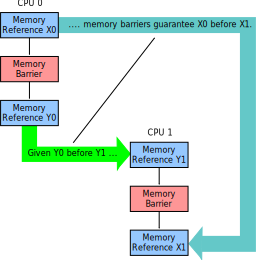
\includegraphics{memorder/memorybarrier}}
\caption{Memory Barriers Provide Conditional If-Then Ordering}
\label{fig:memorder:Memory Barriers Provide Conditional If-Then Ordering}
\end{figure}

\paragraph{Ordering has conditional if-then semantics.}
Figure~\ref{fig:memorder:Memory Barriers Provide Conditional If-Then Ordering}
illustrates this for memory barriers.
Assuming that both memory barriers are strong enough (and when in doubt, you
can always use \co{smp_mb()}), if CPU~1's access Y1 happens after CPU~0's
access Y0, then CPU~1's access X1 is guaranteed to happen after CPU~0's
access X1.

\QuickQuiz{}
	How can you tell which memory barriers are strong enough for
	a given use case?
\QuickQuizAnswer{
	Ah, that is a deep question whose answer requires most of the
	rest of this chapter.
} \QuickQuizEnd

Listing~\ref{lst:memorder:Memory Ordering: Store-Buffering Litmus Test}
is a case in point.
The \co{smp_mb()} on line~10 and~20 serve as the barriers,
the write to \co{x0} on line~9 as X0, the read from \co{x1} on line~11
as Y0, the write to \co{x1} on line~19 as Y1, and the read from
\co{x0} and X1.
Applying the if-then rule step by step, we know that the write to
\co{x1} on line~19 happens after the read from \co{x1} on line~11 if
\co{P0()}'s local variable \co{r2} is set to the value zero.
The if-then rule would then state that the read from \co{x1} on
line~21 happens after the write to \co{x1} on line~9.
In other words,
\co{P1()}'s local variable \co{r2} is guaranteed
to end up with the value two \emph{only if}
\co{P0()}'s local variable \co{r2} ends up with the value zero.
Again, memory ordering guarantees are conditional, not absolute.

Although
Figure~\ref{fig:memorder:Memory Barriers Provide Conditional If-Then Ordering}
specifically mentions memory barriers, the same rule applies to the
rest of the Linux kernel's ordering operations.

\paragraph{Ordering operations must be paired.}
If you carefully order the operations in one thread, but then fail to do
so in another thread, then there is no ordering.
Both threads must provide ordering for the if-then rule to apply.
% @@@ forward reference to cycles.

\paragraph{Ordering operations almost never speed things up.}
If you find yourself tempted to add a memory barrier in an attempt
to force a prior write to be flushed to memory faster, resist!
Adding ordering usually slows things down.
Of course, there are situations where adding instructions speeds things
up, but careful benchmarking is required in such cases.
And even then, it is quite possible that although you sped things up
a little bit on \emph{your} system, you might well have slowed things
down significantly on your users' systems.
Or on your future system.

\paragraph{Ordering operations are not magic.}
When your program is failing due to some race condition, it is often
tempting to toss in a few memory-ordering operations in an attempt
to barrier your bug out of existence.
A far better reaction is to use higher-level primitives in a carefully
designed manner.
With concurrent programming, it is almost always easier to design
your bugs out of existence than to hack them out of existence!

\paragraph{These are only rules of thumb.}
Although these rules of thumb cover the vast majority of situations
seen in actual practice, as with any set of rules of thumb, they
do have their limits.
The next section will demonstrate some of these limits by introducing
trick-and-trap litmus tests that will hopefully both insult your
intuition and increase your understanding.
These litmus tests will also illuminate many of the concepts
represented by
Table~\ref{tab:memorder:Linux-Kernel Memory-Ordering Cheat Sheet}.

\section{Tricks and Traps}
\label{sec:memorder:Tricks and Traps}

Now that you know that hardware can reorder memory accesses and that you
can prevent it from doing so, the next step is to get you to admit
that your intuition has a problem.
This painful task is taken up by
Section~\ref{sec:memorder:Variables With Multiple Values},
which presents some code demonstrating that scalar variables can
take on multiple values simultaneously,
and by
Sections~\ref{sec:memorder:Memory-Reference Reordering} through
\ref{sec:memorder:Multicopy Atomicity},
which show a series of intuitively correct code fragments that fail miserably
on real hardware.
Once your intuition has made it through the grieving process,
Section~\ref{sec:memorder:What Can You Trust?}
provides the basic rules that memory barriers follow, rules that we
will build upon.
These rules are further refined in
Sections~\ref{sec:memorder:Review of Locking Implementations}
through~\ref{sec:memorder:Where Are Memory Barriers Needed?}.

But first, let's take a quick look at just how many values a single
variable might have at a single moment of time.

\subsection{Variables With Multiple Values}
\label{sec:memorder:Variables With Multiple Values}

하나의 변수는 잘 정의된 전역적 순서로 값들의 연속을 갖게 될 거라 생각하는건
자연스럽습니다.
불행히도, 이 여정의 다음 정류장은 이 편안한 거짓에 ``작별''을 고하라 합니다.
바라건대, 여러분은 이미
Tables~\ref{tab:memorder:Memory Misordering: Store-Buffering Sequence of Events}
와~\ref{tab:memorder:Memory Ordering: Store-Buffering Sequence of Events} 의
row~2 를 통해 ``작별'' 을 고하기 시작했을 것이고 만약 그렇다면 이 섹션의 목적은
이 요점을 제대로 이끌어내는 것입니다.
\iffalse

It is natural to think of a variable as taking on a well-defined
sequence of values in a well-defined, global order.
Unfortunately, the next stop on the journey says ``goodbye'' to this comforting fiction.
Hopefully, you already started to say ``goodbye'' in response to row~2 of
Tables~\ref{tab:memorder:Memory Misordering: Store-Buffering Sequence of Events}
and~\ref{tab:memorder:Memory Ordering: Store-Buffering Sequence of Events},
and if so, the purpose of this section is to drive this point home.
\fi

그러기 위해,
Listing~\ref{lst:memorder:Software Logic Analyzer} 에 보인 프로그램의 한 부분을
고려해 봅시다.
이 코드 조각은 여러 CPU 들에서 병렬적으로 수행됩니다.
Line~1 은 하나의 공유 변수를 현재 CPU 의 ID 로 값을 할당하고, line~2 에서는
모든 CPU 들 가운데 동기화 되는 (불행히도, 모든 CPU 구조에서 가능한 일은
아닙니다!) 하드웨어 ``timebase'' 카운터의 값을 가져오는 \co{gettb()} 함수를
사용해 일부 변수들을 초기화 시키고, line~3-8 의 루프에서는 이 CPU 가 할당한
값이 유지된 시간의 길이를 기록합니다.
물론, 이 CPU 들 가운데 하나는 ``승리'' 할 것이고, 따라서 line~6-7 의 검사가
아니라면 이 루프를 절대 빠져나오지 않을 겁니다.
\iffalse

To this end, consider the program fragment shown in
Listing~\ref{lst:memorder:Software Logic Analyzer}.
This code fragment is executed in parallel by several CPUs.
Line~1 sets a shared variable to the current CPU's ID, line~2
initializes several variables from a \co{gettb()} function that
delivers the value of a fine-grained hardware ``timebase'' counter that is
synchronized among all CPUs (not available from all CPU architectures,
unfortunately!), and the loop from lines~3-8 records the length of
time that the variable retains the value that this CPU assigned to it.
Of course, one of the CPUs will ``win'', and would thus never exit
the loop if not for the check on lines~6-7.
\fi

\QuickQuiz{}
	Listing~\ref{lst:memorder:Software Logic Analyzer}
	의 코드에서의 어떤 가정이 실제 하드웨어에서는 성립하지 않을까요?
	\iffalse

	What assumption is the code fragment
	in Listing~\ref{lst:memorder:Software Logic Analyzer}
	making that might not be valid on real hardware?
	\fi
\QuickQuizAnswer{
	이 코드는 특정 CPU 가 자신의 값을 보는 것을 멈추자마자, 곧바로
	마지막으로 동의된 값을 보게 될 것이라 가정삽니다.
	실제 하드웨어에서, 어떤 CPU 들은 이 마지막 값을 보게 되기 전에 중간의
	결과를 일부 보게 될수도 있습니다.
	따라서 이 섹션의 뒤에서 이야기될 그림들의 데이터를 만드는데 사용된 실제
	코드는 좀 더 복잡합니다.
	\iffalse

	The code assumes that as soon as a given CPU stops
	seeing its own value, it will immediately see the
	final agreed-upon value.
	On real hardware, some of the CPUs might well see several
	intermediate results before converging on the final value.
	The actual code used to produce the data in the figures
	discussed later in this section was therefore somewhat more
	complex.
	\fi
} \QuickQuizEnd

\begin{listing}[tbp]
{ \scriptsize
\begin{verbbox}
  1 state.variable = mycpu;
  2 lasttb = oldtb = firsttb = gettb();
  3 while (state.variable == mycpu) {
  4   lasttb = oldtb;
  5   oldtb = gettb();
  6   if (lasttb - firsttb > 1000)
  7     break;
  8 }
\end{verbbox}
}
\centering
\theverbbox
\caption{Software Logic Analyzer}
\label{lst:memorder:Software Logic Analyzer}
\end{listing}

루프를 빠져나오기 전, \co{firsttb} 는 앞의 공유 변수에의 값 할당 후 곧바로
가져온 timestamp 를 가지고 있을 것이고 \co{lasttb} 는 여전히 할당된 값을 가지고
있을, 이 공유 변수의 마지막 샘플링 전에 가져온 timestamp 를 가지고 있을 수도
있고, 만약 이 공유 변수가 루프에 들어오기 전에 바뀌었다면 \co{firsttb} 와 같은
값을 가지고 있을 수도 있습니다.
이는 우리가 532-나노세컨드의 시간 간격 동안의 각 CPU 의 \co{state.variable} 의
값에 대한 관찰을 그려볼 수 있게 해주는데,
Figure~\ref{fig:memorder:A Variable With Multiple Simultaneous Values} 에
보여져 있습니다.
이 데이터는 2006년에 각각 두개의 하드웨어 쓰레드를 갖는 8개의 코어를 장착한
1.5\,GHz POWER5 시스템에서 수집되었습니다.
CPU~1, 2, 3, 그리고~4 는 이 값들을 기록했고, CPU~0 는 이 테스트를 제어했습니다.
Timebase 카운터의 시간 간격은 5.32\,ns 정도였는데, 이는 중간의 캐시 상태들을
관찰하기에 충분히 작은 간격입니다.
\iffalse

Upon exit from the loop, \co{firsttb} will hold a timestamp
taken shortly after the assignment and \co{lasttb} will hold
a timestamp taken before the last sampling of the shared variable
that still retained the assigned value, or a value equal to \co{firsttb}
if the shared variable had changed before entry into the loop.
This allows us to plot each CPU's view of the value of \co{state.variable}
over a 532-nanosecond time period, as shown in
Figure~\ref{fig:memorder:A Variable With Multiple Simultaneous Values}.
This data was collected in 2006 on 1.5\,GHz POWER5 system with 8 cores,
each containing a pair of hardware threads.
CPUs~1, 2, 3, and~4 recorded the values, while CPU~0 controlled the test.
The timebase counter period was about 5.32\,ns, sufficiently fine-grained
to allow observations of intermediate cache states.
\fi

\begin{figure}[htb]
\centering
\resizebox{3in}{!}{\includegraphics{memorder/MoreThanOneValue}}
\caption{A Variable With Multiple Simultaneous Values}
\label{fig:memorder:A Variable With Multiple Simultaneous Values}
\end{figure}

각각의 수평의 막대는 해당 CPU 의 관찰 결과를 시간대별로 보여주는데, 왼쪽 검은
영역은 해당 CPU 의 첫번째 관측 전까지의 시간을 나타냅니다.
처음 5\,ns 동안, CPU~3 만이 이 변수의 값을 읽었습니다.
그 다음 10\,ns 동안, CPU~2 와~3 은 이 변수의 값을 서로 다르게 이야기했는데, 그
후에는 최종적으로 동의된 값인 ``2'' 라는 값에 합의했습니다.
하지만, CPU~1 은 이 값이 ``1'' 이라고 거의 300\,ns 동안 믿었고, CPU~4 는 거의
500\,ns 동안이나 이 값이 ``4'' 라고 믿었습니다.
\iffalse

Each horizontal bar represents the observations of a given CPU over time,
with the black regions to the left indicating the time before the
corresponding CPU's first measurement.
During the first 5\,ns, only CPU~3 has an opinion about the value of the
variable.
During the next 10\,ns, CPUs~2 and~3 disagree on the value of the variable,
but thereafter agree that the value is~``2'', which is in fact
the final agreed-upon value.
However, CPU~1 believes that the value is~``1'' for almost 300\,ns, and
CPU~4 believes that the value is~``4'' for almost 500\,ns.
\fi

\QuickQuiz{}
	어떻게 CPU 들이 하나의 변수를 \emph{동시에} 서로 다르게 볼 수가
	있는거죠?
	\iffalse

	How could CPUs possibly have different views of the
	value of a single variable \emph{at the same time?}
	\fi
\QuickQuizAnswer{
	Section~\ref{sec:memorder:Why Hardware Misordering?}
	에서 논의된 대로, 많은 CPU 들이 최근의 쓰기 값을 기록하는 쓰기 버퍼를
	가지고 있으며, 이 값은 연관된 캐시 라인이 해당 CPU 로 올라왔을 때에
	적용됩니다.
	따라서, 각 CPU 가 하나의 시점에 특정 변수에 대해 서로 다른 값을 보고
	있는 것이---그리고 메인 메모리는 또 다른 값을 가지고 있는 것이
	가능합니다.
	메모리 배리어가 발명된 이유들 중 하나는 소프트웨어가 이런 종류의 상황을
	우아하게 처리할 수 있도록 해주기 위함이었습니다.
	\iffalse

	As discussed in
	Section~\ref{sec:memorder:Why Hardware Misordering?},
	many CPUs have write buffers that record the values of
	recent writes, which are applied once the corresponding
	cache line makes its way to the CPU.
	Therefore, it is quite possible for each CPU to see a
	different value for a given variable at a single point
	in time---and for main memory to hold yet another value.
	One of the reasons that memory barriers were invented was
	to allow software to deal gracefully with situations like
	this one.
	\fi
} \QuickQuizEnd

\QuickQuiz{}
	CPU~1 과~4 는 값을 동의하는데에 그렇게 오랜 시간이 걸렸는데, CPU~2 와~3
	은 어떻게 그렇게 빨리 값에 동의하는 건가요?
	\iffalse

	Why do CPUs~2 and~3 come to agreement so quickly, when it
	takes so long for CPUs~1 and~4 to come to the party?
	\fi
\QuickQuizAnswer{
	CPU~2 와~3 은 같은 코어의 하드웨어 쓰레드들이어서 같은 캐시 계층을
	공유하며, 따라서 매우 낮은 통신 응답시간을 갖습니다.
	이게 NUMA, 또는, 보다 정확히는, NUCA 효과입니다.

	이는 CPU~2 와~3 가 왜 값에 대해 동의하지 않는 순간이 존재하긴 하는가에
	대한 질문을 떠올리게 합니다.
	가능한 한가지 이유는 이들이 커다란 공유된 캐시 외에 작은 개별 캐시를
	갖고 있을 수 있다는 것입니다.
	여기서의 짧은 10-나노세컨드 동안의 비동의된 시간과 해당 코드에 메모리
	배리어가 아예 없었다는 것을 놓고 보면, 또다른 가능할 법한 이유는
	인스트럭션 재배치입니다.
	\iffalse

	CPUs~2 and~3 are a pair of hardware threads on the same
	core, sharing the same cache hierarchy, and therefore have
	very low communications latencies.
	This is a NUMA, or, more accurately, a NUCA effect.

	This leads to the question of why CPUs~2 and~3 ever disagree
	at all.
	One possible reason is that they each might have a small amount
	of private cache in addition to a larger shared cache.
	Another possible reason is instruction reordering, given the
	short 10-nanosecond duration of the disagreement and the
	total lack of memory barriers in the code fragment.
	\fi
} \QuickQuizEnd

그리고 네개의 CPU 에서의 상황이 재밌다고 생각한다면, 같은 상황을 15~CPU 들이
각각 시간 $t=0$ 에 하나의 공유 변수에 각자의 숫자를 할당하는 경우를 보인
Figure~\ref{fig:memorder:A Variable With More Simultaneous Values} 를 고려해
보세요.
해당 그림의 두 다이어그램은 모두
Figure~\ref{fig:memorder:A Variable With Multiple Simultaneous Values} 와 같은
방식으로 그려졌습니다.
유일한 차이점은 가로축의 단위가 timebase tick 으로, 각 tick 은 약
5.3~나노세컨드를 의미합니다.
따라서 여기서의 전체 연속된 값의 변화는 CPU 의 수의 증가에 일관되게
Figure~\ref{fig:memorder:A Variable With Multiple Simultaneous Values} 에서보다
긴 시간동안 유지되었습니다.
위의 다이어그램은 전체 그림을 보이며, 아래쪽의 것은 첫 50~timebase tick 만을
확대해서 보입니다.

여기서도, CPU~0 는 테스트를 제어했고, 따라서 어떤 값도 기록하지 않았습니다.
\iffalse

And if you think that the situation with four CPUs was intriguing, consider
Figure~\ref{fig:memorder:A Variable With More Simultaneous Values},
which shows the same situation, but with 15~CPUs each assigning their
number to a single shared variable at time~$t=0$. Both diagrams in the
figure are drawn in the same way as 
Figure~\ref{fig:memorder:A Variable With Multiple Simultaneous Values}.
The only difference is that the unit of horizontal axis is timebase ticks,
with each tick lasting about 5.3~nanoseconds.
The entire sequence therefore lasts a bit longer than the events recorded in
Figure~\ref{fig:memorder:A Variable With Multiple Simultaneous Values},
consistent with the increase in number of CPUs.
The upper diagram shows the overall picture, while the lower one shows
the zoom-up of first 50~timebase ticks.

Again, CPU~0 coordinates the test, so does not record any values.
\fi

\begin{figure*}
\centering
\resizebox{5in}{!}{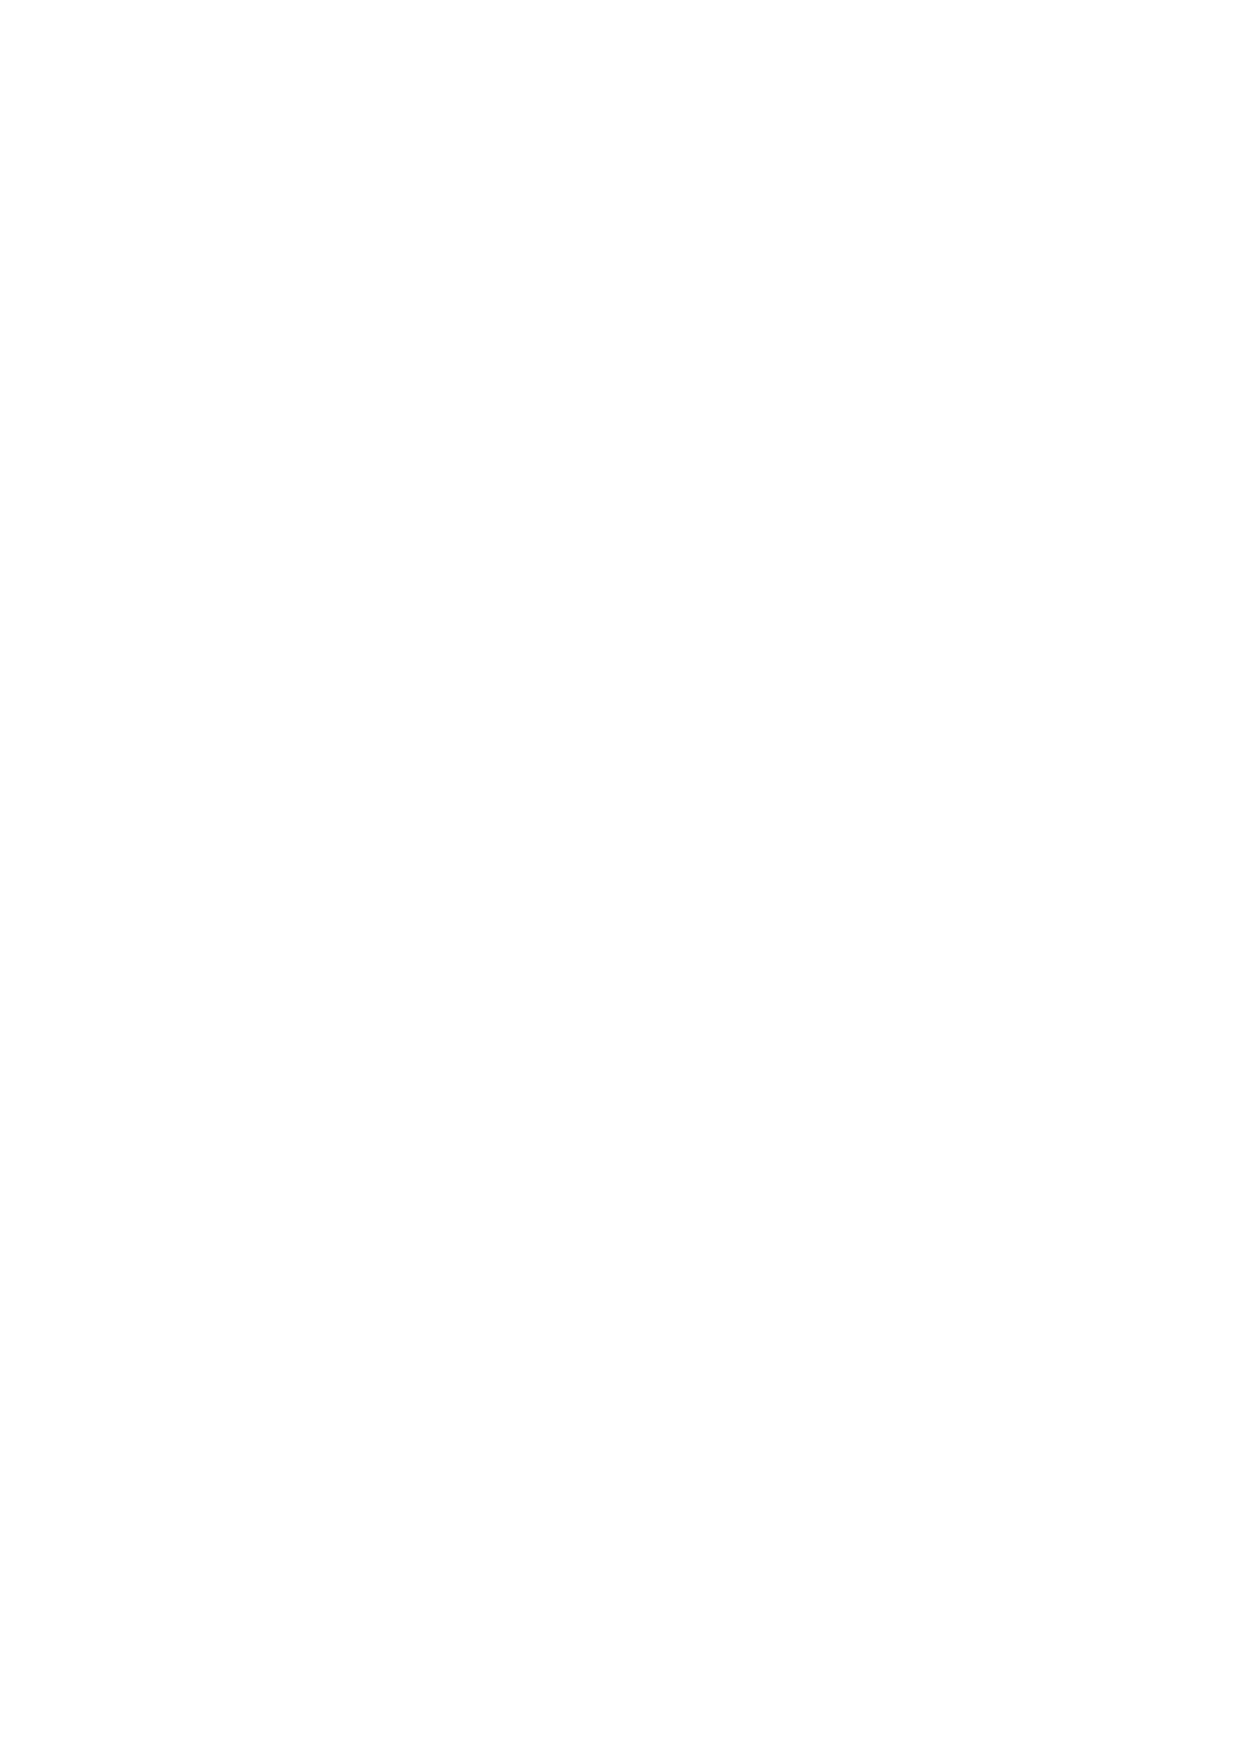
\includegraphics{memorder/MoreThanOneValue-15CPU}}
\caption{A Variable With More Simultaneous Values}
\ContributedBy{Figure}{fig:memorder:A Variable With More Simultaneous Values}{Akira Yokosawa}
\end{figure*}

모든 CPU 들이 결국은 마지막 값~9 에 동의를 합니다만, 값~15 와 값~12 가 먼저
상황을 이끈 후입니다.
아래쪽 다이어그램의 수직선으로 나타내어진 time~21 시점에 변수의 값에 대한
14개의 서로 다른 의견들이 존재했음을 알아두시기 바랍니다.
또한 모든 CPU 들이 값들의 순서에 대해
Figure~\ref{fig:memorder:Possible Global Orders With More Simultaneous Values}
에 보인 방향성 있는 그래프의 순서와 일관된 순서를 보았음을 알아두시기 바랍니다.
더도 아니고 덜도 아니고, 두 그림은 메모리 접근 순서에 신경 쓰는 코드에서의
메모리 배리어의 올바른 사용의 중요성을 강조합니다.
\iffalse

All CPUs eventually agree on the final value of~9, but not before
the values~15 and~12 take early leads.
Note that there are fourteen different opinions on the variable's value
at time~21 indicated by the vertical line in the lower diagram.
Note also that all CPUs see sequences whose orderings are consistent with
the directed graph shown in
Figure~\ref{fig:memorder:Possible Global Orders With More Simultaneous Values}.
Nevertheless, both figures underscore the importance of
proper use of memory barriers for code that cares about memory ordering.
\fi

\begin{figure}[htb]
\centering
\resizebox{2.5in}{!}{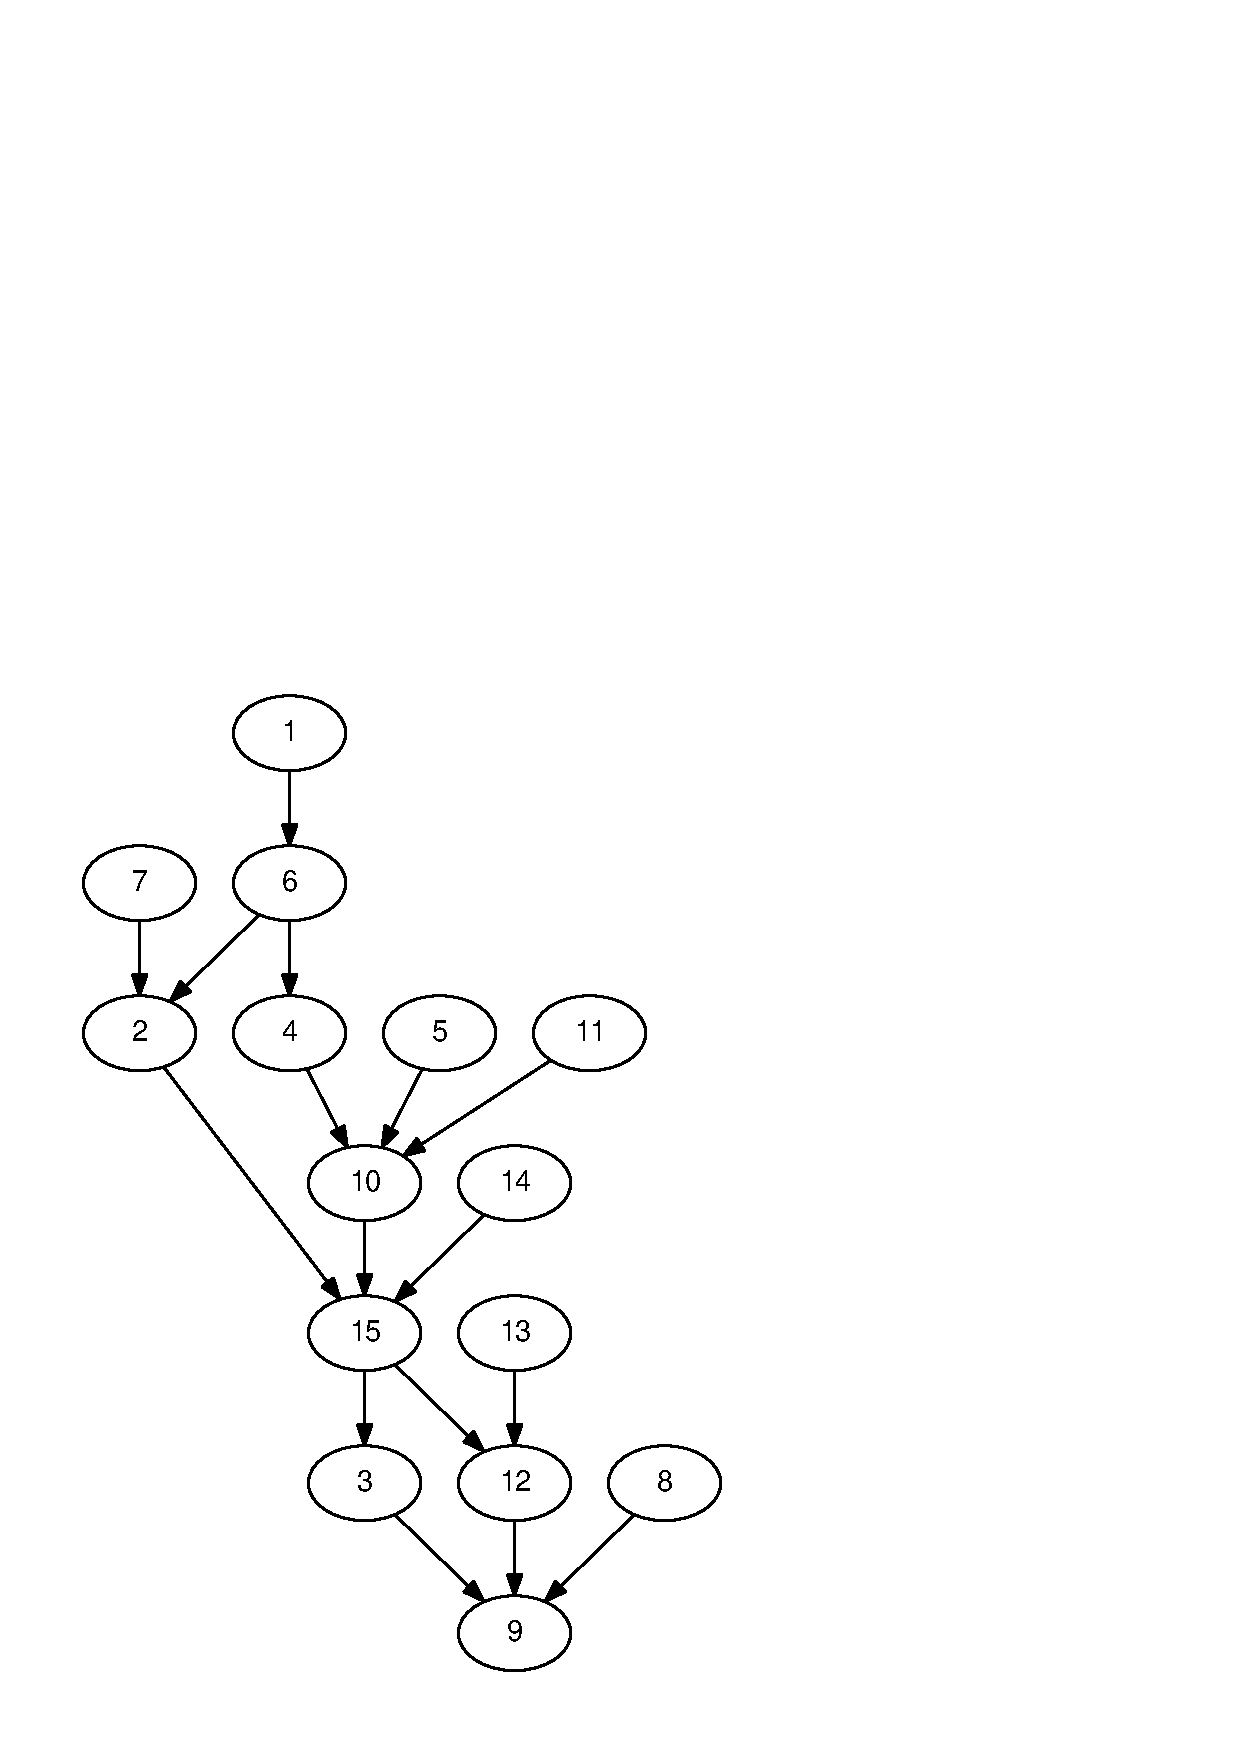
\includegraphics{memorder/store15tred}}
\caption{Possible Global Orders With More Simultaneous Values}
\label{fig:memorder:Possible Global Orders With More Simultaneous Values}
\end{figure}

하나의 변수는 한 시점에 얼마나 많은 값들을 가질 수 있을까요?
시스템에 존재하는 스토어 버퍼 하나당 하나씩입니다!
따라서 우리는 변수들의 값들과 시간의 흐름에 대한 편안한 직관에게 작별을
고해야만 하는 체제에 들어섰습니다.
이는 메모리 배리어들이 필요한 체제입니다.

이와 함께,
Chapter~\ref{chp:Hardware and its Habits}
와~\ref{cha:Partitioning and Synchronization Design} 에서 배웠던 교훈들을
기억할 필요가 있습니다.
모든 CPU 들이 같은 변수에게 동시에 쓰기를 하도록 하는 것은 병렬 프로그램을
설계하는 방법이 아닌데, 적어도 성능과 확장성이 여러분에게 전혀 중요하지 않은 게
아니라면 그렇습니다.

불행히도, 메모리 순서 규칙은 여러분의 직관을 망칠 수 있는 방법들을 이외에도
많이 가지고 있으며, 이런 방법들 모두가 성능과 확장성을 훼손하는 건 아닙니다.
다음 섹션은 관계없는 메모리 참조의 순서 재배치에 대한 소개를 제공합니다.
\iffalse

How many values can a single variable take on at a single point in
time?
As many as one per store buffer in the system!
We have therefore entered a regime where we must bid a fond farewell to
comfortable intuitions about values of variables and the passage of time.
This is the regime where memory barriers are needed.

All that aside, it is important to remember the lessons from
Chapters~\ref{chp:Hardware and its Habits}
and~\ref{cha:Partitioning and Synchronization Design}.
Having all CPUs write concurrently to the same variable
is absolutely no way to design a parallel program, at least
not if performance and scalability are at all important to you.

Unfortunately, memory ordering has many other ways of insulting your
intuition, and not all of these ways conflict with performance and
scalability.
The next section will give an overview of reordering of unrelated
memory reference.
\fi

\subsection{Memory-Reference Reordering}
\label{sec:memorder:Memory-Reference Reordering}

Section~\ref{sec:memorder:Why Hardware Misordering?}
showed that even relatively strongly ordered systems like x86
can reorder prior stores with later loads, at least when the
store and load are to different variables.
This section builds on that result, looking at the other combinations of
loads and stores.

% @@@ Rationale for further reordering.

\begin{listing}[tbp]
{ \scriptsize
\begin{verbbox}[\LstLineNo]
C C-MP+o-wmb-o+o-o

{
}


P0(int* x0, int* x1) {

  WRITE_ONCE(*x0, 2);
  smp_wmb();
  WRITE_ONCE(*x1, 2);

}

P1(int* x0, int* x1) {

  int r2;
  int r3;

  r2 = READ_ONCE(*x1);
  r3 = READ_ONCE(*x0);

}

exists (1:r2=2 /\ 1:r3=0)
\end{verbbox}
}
\centering
\theverbbox
\caption{Message-Passing Litmus Test (No Ordering)}
\label{lst:memorder:Message-Passing Litmus Test (No Ordering)}
\end{listing}

\subsubsection{Load Followed By Load}
Listing~\ref{lst:memorder:Message-Passing Litmus Test (No Ordering)}
(\path{C-MP+o-wmb-o+o-o.litmus})
shows the classic \emph{message-passing} litmus test, where \co{x0} is
the message and \co{x1} is a flag indicating whether or not a message
is available.
In this test, the \co{smp_wmb()} forces \co{P0()} writes to be ordered,
but no ordering is specified for the reads.
Relatively strongly ordered architectures, such as x86, do enforce ordering.
However, weakly ordered architectures often do
not~\cite{JadeAlglave2011ppcmem}.
Therefore, the \co{exists} clause on line~25 of the listing \emph{can}
trigger.

\begin{listing}[tbp]
{ \scriptsize
\begin{verbbox}[\LstLineNo]
C C-MP+o-wmb-o+o-rmb-o

{
}

P0(int* x0, int* x1) {

  WRITE_ONCE(*x0, 2);
  smp_wmb();
  WRITE_ONCE(*x1, 2);

}

P1(int* x0, int* x1) {

  int r2;
  int r3;

  r2 = READ_ONCE(*x1);
  smp_rmb();
  r3 = READ_ONCE(*x0);

}

exists (1:r2=2 /\ 1:r3=0)
\end{verbbox}
}
\centering
\theverbbox
\caption{Enforcing Order of Message-Passing Litmus Test}
\label{lst:memorder:Enforcing Order of Message-Passing Litmus Test}
\end{listing}

Therefore, portable code relying on ordering in this case should
add explicit ordering, for example, the \co{smp_rmb()} shown on
line~20 of
Listing~\ref{lst:memorder:Enforcing Order of Message-Passing Litmus Test}
(\path{C-MP+o-wmb-o+o-rmb-o.litmus}).
Here, the \co{exists} clause cannot trigger.

\begin{listing}[tbp]
{ \scriptsize
\begin{verbbox}[\LstLineNo]
C C-LB+o-o+o-o
{
}

P0(int *x0, int *x1)
{
  int r2;

  r2 = READ_ONCE(*x1);
  WRITE_ONCE(*x0, 2);
}


P1(int *x0, int *x1)
{
  int r2;

  r2 = READ_ONCE(*x0);
  WRITE_ONCE(*x1, 2);
}

exists (1:r2=2 /\ 0:r2=2)
\end{verbbox}
}
\centering
\theverbbox
\caption{Load-Buffering Litmus Test (No Ordering)}
\label{lst:memorder:Load-Buffering Litmus Test (No Ordering)}
\end{listing}

\subsubsection{Load Followed By Store}
Listing~\ref{lst:memorder:Load-Buffering Litmus Test (No Ordering)}
(\path{C-LB+o-o+o-o.litmus}),
shows the classic \emph{load-buffering} litmus test.
Although relatively strongly ordered systems such as x86
or the IBM Mainframe do not reorder prior loads with subsequent stores,
more weakly ordered architectures really do allow such
reordering~\cite{JadeAlglave2011ppcmem}.
Therefore, the \co{exists} clause on line~22 really can trigger.

\begin{listing}[tbp]
{ \scriptsize
\begin{verbbox}[\LstLineNo]
C C-LB+o-r+a-o
{
}

P0(int *x0, int *x1)
{
  int r2;

  r2 = READ_ONCE(*x1);
  smp_store_release(x0, 2);
}


P1(int *x0, int *x1)
{
  int r2;

  r2 = smp_load_acquire(x0);
  WRITE_ONCE(*x1, 2);
}

exists (1:r2=2 /\ 0:r2=2)
\end{verbbox}
}
\centering
\theverbbox
\caption{Enforcing Ordering of Load-Buffering Litmus Test}
\label{lst:memorder:Enforcing Ordering of Load-Buffering Litmus Test}
\end{listing}

Interestingly enough, it is relatively rare for actual hardware to
exhibit this reordering~\cite{LucMaranget2017aarch64}.
Nevertheless, you should enforce any required ordering, for example,
as shown in
Listing~\ref{lst:memorder:Enforcing Ordering of Load-Buffering Litmus Test}
(\path{C-LB+o-r+a-o.litmus}),
thus guaranteeing that the \co{exists} clause on line~22 never triggers.

\begin{listing}[tbp]
{ \scriptsize
\begin{verbbox}[\LstLineNo]
C C-MP+o-o+o-rmb-o

{
}

P0(int* x0, int* x1) {

  WRITE_ONCE(*x0, 2);
  WRITE_ONCE(*x1, 2);

}

P1(int* x0, int* x1) {

  int r2;
  int r3;

  r2 = READ_ONCE(*x1);
  smp_rmb();
  r3 = READ_ONCE(*x0);

}

exists (1:r2=2 /\ 1:r3=0)
\end{verbbox}
}
\centering
\theverbbox
\caption{Message-Passing Litmus Test, No Writer Ordering (No Ordering)}
\label{lst:memorder:Message-Passing Litmus Test, No Writer Ordering (No Ordering)}
\end{listing}

\subsubsection{Store Followed By Store}
Listing~\ref{lst:memorder:Message-Passing Litmus Test, No Writer Ordering (No Ordering)}
(\path{C-MP+o-o+o-rmb-o.litmus})
once again shows the classic message-passing litmus test, but without
explicit ordering for \co{P0()}'s writes and with the \co{smp_rmb()}
providing ordering for \co{P1()}'s reads.
Again, the relatively strongly ordered architectures do enforce ordering,
but weakly ordered architectures do not necessarily do
so~\cite{JadeAlglave2011ppcmem}, which means that the
\co{exists} clause can trigger.
Therefore, portable code should explicitly order the writes, for
example, as shown in
Listing~\ref{lst:memorder:Enforcing Order of Message-Passing Litmus Test},
thus preventing the \co{exists} clause from triggering.

\subsection{Address Dependencies}
\label{sec:memorder:Address Dependencies}

An \emph{address dependency} occurs when the value returned by a load
instruction is used to compute the address used by a later memory-reference
instruction.

\begin{listing}[tbp]
{ \scriptsize
\begin{verbbox}[\LstLineNo]
C C-MP+o-wmb-o+o-addr-o

{
int y=1;
int *x1 = &y;
}

P0(int* x0, int** x1) {

  WRITE_ONCE(*x0, 2);
  smp_wmb();
  WRITE_ONCE(*x1, x0);

}

P1(int** x1) {

  int *r2;
  int r3;

  r2 = READ_ONCE(*x1);
  r3 = READ_ONCE(*r2);

}

exists (1:r2=x0 /\ 1:r3=1)
\end{verbbox}
}
\centering
\theverbbox
\caption{Message-Passing Address-Dependency Litmus Test (No Ordering)}
\label{lst:memorder:Message-Passing Address-Dependency Litmus Test (No Ordering)}
\end{listing}

Listing~\ref{lst:memorder:Message-Passing Address-Dependency Litmus Test (No Ordering)}
(\path{C-MP+o-wmb-o+o-addr-o.litmus}),
shows a linked variant of the message-passing pattern.
The head pointer is \co{x1}, which initially
references the \co{int} variable \co{y} (line~5), which is in turn 
initialized to the value $1$ (line~4).
\co{P0()} updates head pointer \co{x1} to reference \co{x0} (line~12),
but only afer initializing it to $2$ (line~10) and forcing ordering
(line~11).
\co{P1()} picks up the head pointer \co{x1} (line~21), and then loads
the referenced value (line~22).
There is thus an address dependency from the load on line~21 to the
load on line~22.
In this case, the value returned by line~21 is exactly the address
used by line~22, but many variations are possible,
including field access using the C-language \co{->} operator,
addition, subtraction, and array indexing.

One might hope that line~21's load from the head pointer would be ordered
before line~22's dereference.
However, this is not the case on DEC Alpha, which can in effect use
a speculated value for the dependent read, as described in more detail in
Section~\ref{sec:app:whymb:Alpha}.
Therefore,
Listing~\ref{lst:memorder:Message-Passing Address-Dependency Litmus Test (No Ordering)}'s
\co{exists} clause \emph{can} trigger.

\begin{listing}[tbp]
{ \scriptsize
\begin{verbbox}[\LstLineNo]
C C-MP+o-wmb-o+ld-addr-o

{
int y=1;
int *x1 = &y;
}

P0(int* x0, int** x1) {

  WRITE_ONCE(*x0, 2);
  smp_wmb();
  WRITE_ONCE(*x1, x0);

}

P1(int** x1) {

  int *r2;
  int r3;

  r2 = lockless_dereference(*x1);
  r3 = READ_ONCE(*r2);

}

exists (1:r2=x0 /\ 1:r3=1)
\end{verbbox}
}
\centering
\theverbbox
\caption{Enforced Ordering of Message-Passing Address-Dependency Litmus Test}
\label{lst:memorder:Enforced Ordering of Message-Passing Address-Dependency Litmus Test}
\end{listing}

Listing~\ref{lst:memorder:Enforced Ordering of Message-Passing Address-Dependency Litmus Test}
(\path{C-MP+o-wmb-o+ld-addr-o.litmus})
shows how to make this work portably, even on DEC Alpha, by
replacing line~21's \co{READ_ONCE()} with \co{lockless_dereference()},
which acts like \co{READ_ONCE()} on all platforms other than DEC Alpha,
where it acts like a \co{READ_ONCE()} followed by an \co{smp_mb()},
thereby forcing the required ordering on all platforms, in turn
preventing the \co{exists} clause from triggering.

\begin{listing}[tbp]
{ \scriptsize
\begin{verbbox}[\LstLineNo]
C C-S+o-wmb-o+o-addr-o

{
int y=1;
int *x1 = &y;
}

P0(int* x0, int** x1) {

  WRITE_ONCE(*x0, 2);
  smp_wmb();
  WRITE_ONCE(*x1, x0);

}

P1(int** x1) {

  int *r2;

  r2 = READ_ONCE(*x1);
  WRITE_ONCE(*r2, 3);

}

exists (1:r2=x0 /\ x0=2)
\end{verbbox}
}
\centering
\theverbbox
\caption{S Address-Dependency Litmus Test}
\label{lst:memorder:S Address-Dependency Litmus Test}
\end{listing}

But what happens if the dependent operation is a write rather than
a read, for example, in the \emph{S}
litmus test~\cite{JadeAlglave2011ppcmem} shown in
Listing~\ref{lst:memorder:S Address-Dependency Litmus Test}
(\path{C-S+o-wmb-o+o-addr-o.litmus})?
Because no production-quality platform speculates writes,
it is not possible for the \co{WRITE_ONCE()} on line~10 to overwrite
the \co{WRITE_ONCE()} on line~21, meaning that the \co{exists}
clause on line~25 cannot trigger, even on DEC Alpha, even
without the \co{lockless_dereference()} that is required in the
dependent-read case.

\QuickQuiz{}
	But how do we know that \emph{all} platforms really avoid
	triggering the \co{exists} clauses in
	Listings~\ref{lst:memorder:Enforced Ordering of Message-Passing Address-Dependency Litmus Test}
	and~\ref{lst:memorder:S Address-Dependency Litmus Test}?
\QuickQuizAnswer{
	Answering this requires identifying three major groups of platforms:
	(1)~Total-store-order (TSO) platforms,
	(2)~Weakly ordered platorms, and
	(3)~DEC Alpha.

	The TSO platforms order all pairs of memory references except for
	prior stores against later loads.
	Because the address dependency on lines~21 and ~22 of
	Listing~\ref{lst:memorder:Enforced Ordering of Message-Passing Address-Dependency Litmus Test}
	is instead a load followed by another load, TSO platforms preserve
	this address dependency.
	They also preserve the address dependency on lines~20 and~21 of
	Listing~\ref{lst:memorder:S Address-Dependency Litmus Test}
	because this is a load followed by a store.
	Because address dependencies must start with a load, TSO platforms
	implicitly but completely respect them.

	Weakly ordered platforms don't necessarily maintain ordering of
	unrelated accesses.
	However, the address dependencies in
	Listings~\ref{lst:memorder:Enforced Ordering of Message-Passing Address-Dependency Litmus Test}
	and~\ref{lst:memorder:S Address-Dependency Litmus Test}
	are not unrelated: There is an address dependency.
	The hardware tracks dependencies and maintains the needed
	ordering.

	There is one (famous) exception to this rule for weakly ordered
	platforms, and that exception is DEC Alpha for read-to-read
	address dependencies.
	And this is why DEC Alpha requires the explicit memory barrier
	supplied for it by the \co{lockless_dereference()} on line~21 of
	Listings~\ref{lst:memorder:Enforced Ordering of Message-Passing Address-Dependency Litmus Test}.
	However, DEC Alpha does track read-to-write address dependencies,
	which is why line~20 of
	Listings~\ref{lst:memorder:S Address-Dependency Litmus Test}
	does not have a \co{lockless_dereference()}.

	To sum up, current platforms either respect address dependencies
	implicitly, as is the case for TSO platforms (x86, mainframe,
	SPARC,~...), have hardware tracking for address dependencies
	(ARM, PowerPC, MIPS,~...), or have the required memory barriers
	supplied by \co{lockless_dereference()} (DEC Alpha).
} \QuickQuizEnd

However, it is important to note that address dependencies can
be fragile and easily broken by compiler optimizations, as discussed in
Section~\ref{sec:memorder:Address- and Data-Dependency Restrictions}.

\subsection{Data Dependencies}
\label{sec:memorder:Data Reordering}

A \emph{data dependency} occurs when the value returned by a load
instruction is used to compute the data stored by a later store
instruction.
Note well the ``data'' above: If the value returned by a load
was instead used to compute the address used by a later store
instruction, that would instead be an address dependency.

\begin{listing}[tbp]
{ \scriptsize
\begin{verbbox}[\LstLineNo]
C C-LB+o-r+o-data-o
{
}

P0(int *x0, int *x1)
{
  int r2;

  r2 = READ_ONCE(*x1);
  smp_store_release(x0, 2);
}


P1(int *x0, int *x1)
{
  int r2;

  r2 = READ_ONCE(*x0);
  WRITE_ONCE(*x1, r2);
}

exists (1:r2=2 /\ 0:r2=2)
\end{verbbox}
}
\centering
\theverbbox
\caption{Load-Buffering Data-Dependency Litmus Test}
\label{lst:memorder:Load-Buffering Data-Dependency Litmus Test}
\end{listing}

Listing~\ref{lst:memorder:Load-Buffering Data-Dependency Litmus Test}
(\path{C-LB+o-r+o-data-o.litmus})
is similar to
Listing~\ref{lst:memorder:Enforcing Ordering of Load-Buffering Litmus Test},
except that \co{P1()}'s ordering between lines~18 and~19 is
enforced not by an acquire load, but instead by a data dependency:
The value loaded by line~18 is what line~19 stores.
The ordering provided by this data dependency is sufficient to prevent
the \co{exists} clause from triggering.

\QuickQuiz{}
	Why doesn't line~18 of
	Listing~\ref{lst:memorder:Load-Buffering Data-Dependency Litmus Test}
	need a \co{lockless_dereference()}?
\QuickQuizAnswer{
	Data dependencies are always load-to-store dependencies, and
	so all platforms respect them, even DEC Alpha, and for the
	same reasons that they respect load-to-store address dependencies.
} \QuickQuizEnd

Just as with address dependencies, it is important to note that
data dependencies can
be fragile and easily broken by compiler optimizations, as discussed in
Section~\ref{sec:memorder:Address- and Data-Dependency Restrictions}.
In fact, data dependencies can be even more fragile than are address
dependencies.
The reason for this is that address dependencies normally involve
pointer values.
In contrast, as shown in
Listing~\ref{lst:memorder:Load-Buffering Data-Dependency Litmus Test},
it is tempting to carry data dependencies through integral values,
which the compiler has much more freedom to optimize into nonexistence.
For but one example, if the integer loaded was multiplied by the constant
zero, the compiler would know that the result was zero, and could therefore
substitute the constant zero for the value loaded, thus breaking
the dependency.

\QuickQuiz{}
	But wait!!!
	Line~18 of
	Listing~\ref{lst:memorder:Load-Buffering Data-Dependency Litmus Test}
	uses \co{READ_ONCE()}, which marks the load as volatile,
	which means that the compiler absolutely must emit the load
	instruction even if the value is later multiplied by zero.
	So do you really need to work so hard to keep the compiler from
	breaking your data dependencies?
\QuickQuizAnswer{
	Yes, the compiler absolutely must emit a load instruction for
	a volatile load.
	But if you multiply the value loaded by zero, the compiler is
	well within its rights to substitute a constant zero for the
	result of that multiplication, which will break the data
	dependency on many platforms.

	Worse yet, if the dependent store does not use \co{WRITE_ONCE()},
	the compiler could hoist it above the load, which would cause
	even TSO platforms to fail to provide ordering.
} \QuickQuizEnd

In short, you can rely on data dependencies, but only if you take care
to prevent your compiler from breaking them.

\subsection{Control Dependencies}
\label{sec:memorder:Control Dependencies}

A \emph{control dependency} occurs when the value returned by a load
instruction is tested to determine whether or not a later store instruction
is executed.
Note well the ``later store instruction'': Many platforms do not respect
load-to-load control dependencies.

\begin{listing}[tbp]
{ \scriptsize
\begin{verbbox}[\LstLineNo]
C C-LB+o-r+o-ctrl-o
{
}

P0(int *x0, int *x1)
{
  int r2;

  r2 = READ_ONCE(*x1);
  smp_store_release(x0, 2);
}


P1(int *x0, int *x1)
{
  int r2;

  r2 = READ_ONCE(*x0);
  if (r2 >= 0)
    WRITE_ONCE(*x1, 2);
}

exists (1:r2=2 /\ 0:r2=2)
\end{verbbox}
}
\centering
\theverbbox
\caption{Load-Buffering Control-Dependency Litmus Test}
\label{lst:memorder:Load-Buffering Control-Dependency Litmus Test}
\end{listing}

Listing~\ref{lst:memorder:Load-Buffering Control-Dependency Litmus Test}
(\path{C-LB+o-r+o-ctrl-o.litmus}),
shows another load-buffering example, this time using a control
dependency (line~19) to order the load on line~18 and the store on
line~20.
The ordering is sufficient to prevent the \co{exists} from triggering.

However, control dependencies are even more susceptible to being optimized
out of existence than are data dependencies, and
Section~\ref{sec:memorder:Control-Dependency Restrictions}
describes some of the rules that must be followed in order to prevent
your compiler from breaking your control dependencies.

\begin{listing}[tbp]
{ \scriptsize
\begin{verbbox}[\LstLineNo]
C C-MP+o-r+o-ctrl-o

{
}

P0(int* x0, int* x1) {

  WRITE_ONCE(*x0, 2);
  smp_store_release(x1, 2);

}

P1(int* x0, int* x1) {
  int r2;
  int r3;

  r2 = READ_ONCE(*x1);
  if (r2 >= 0)
    r3 = READ_ONCE(*x0);

}

exists (1:r2=2 /\ 1:r3=0)
\end{verbbox}
}
\centering
\theverbbox
\caption{Message-Passing Control-Dependency Litmus Test (No Ordering)}
\label{lst:memorder:Message-Passing Control-Dependency Litmus Test (No Ordering)}
\end{listing}

It is worth reiterating that control dependencies provide ordering only
from loads to stores.
Therefore, the load-to-load control dependency shown on lines~17-19 of
Listing~\ref{lst:memorder:Message-Passing Control-Dependency Litmus Test (No Ordering)}
(\path{C-MP+o-r+o-ctrl-o.litmus})
does \emph{not} provide ordering, and therefore does \emph{not}
prevent the \co{exists} clause from triggering.

In summary, control dependencies can be useful, but they are high
maintenance.
You should therefore use them only when performance considerations
permit no other solution.

\subsection{Cache Coherence}
\label{sec:memorder:Cache Coherence}

On cache-coherent platforms, all CPUs agree on the order of loads and
stores to a given variable.
Fortunately, when \co{READ_ONCE()} and \co{WRITE_ONCE()} are used,
almost all platforms are cache-coherent.
Unfortunately, this property is so popular that it has been named
multiple times, with ``single-variable SC'',\footnote{
	Recall that SC stands for sequentially consistent.}
``single-copy atomic''~\cite{Stone:1995:SP:623262.623912},
and just plain ``coherence''~\cite{JadeAlglave2011ppcmem}
having seen use.
Rather than further compound the confusion by inventing yet another term
for this concept, this book uses ``cache coherence'' and ``coherence''
interchangeably.

\begin{listing}[tbp]
{ \scriptsize
\begin{verbbox}[\LstLineNo]
C C-CCIRIW+o+o+o-o+o-o

{
int x = 0;
}

P0(int *x)
{
  WRITE_ONCE(*x, 1);
}

P1(int *x)
{
  WRITE_ONCE(*x, 2);
}

P2(int *x)
{
  int r1;
  int r2;

  r1 = READ_ONCE(*x);
  r2 = READ_ONCE(*x);
}

P3(int *x)
{
  int r3;
  int r4;

  r3 = READ_ONCE(*x);
  r4 = READ_ONCE(*x);
}

exists(2:r1=1 /\ 2:r2=2 /\ 3:r3=2 /\ 3:r4=1)
\end{verbbox}
}
\centering
\theverbbox
\caption{Cache-Coherent IRIW Litmus Test}
\label{lst:memorder:Cache-Coherent IRIW Litmus Test}
\end{listing}

Listing~\ref{lst:memorder:Cache-Coherent IRIW Litmus Test}
shows a litmus test that tests for cache coherence
(\path{C-CCIRIW+o+o+o-o+o-o.litmus}), where ``IRIW'' stands
for ``independent reads of independent writes''.
Because this litmus test uses only one variable,
\co{P2()} and \co{P3()} must agree
on the order of \co{P0()}'s and \co{P()}'s stores.
In other words, if \co{P2()} believes that \co{P0()}'s store
came first, then \co{P3()} had better not believe that
\co{P1()}'s store came first.
And in fact the \co{exists} clause on line~35 will trigger if this
situation arises.

It is tempting to speculate that different-sized overlapping loads 
and stores to a single region of memory (as might be set up using
the C-language \co{union} keyword) would provide similar ordering
guarantees.
However, Flur et al.~discovered some surprisingly simple
litmus tests that demonstrate that these guarantees can be violated on
real hardware~\cite{Flur:2017:MCA:3093333.3009839}.
It is therefore necessary to restrict code to non-overlapping
same-sized aligned accesses to a given variable, at least if portability
is a consideration.\footnote{
	There is reason to believe that using atomic RMW operations
	(for example, \co{xchg()}) for all the stores will
	provide sequentially consistent ordering, but this has not
	yet been proven either way.}

Adding more variables and threads increases the scope for reordering
and other counterintuitive behavior, as discussed in the next section.

\subsection{Multicopy Atomicity}
\label{sec:memorder:Multicopy Atomicity}

\begin{figure}[tb]
\centering
\resizebox{3.0in}{!}{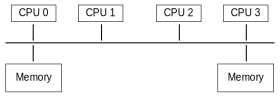
\includegraphics{memorder/SystemArchBus}}
\caption{Global System Bus And Multi-Copy Atomicity}
\label{fig:memorder:Global System Bus And Multi-Copy Atomicity}
\end{figure}

Threads running on a \emph{multicopy atomic}~\cite{Stone:1995:SP:623262.623912}
platform are guaranteed
to agree on the order of writes, even to different variables.
A useful mental model of such a system is the single-bus architecture
shown in
Figure~\ref{fig:memorder:Global System Bus And Multi-Copy Atomicity}.
If each write resulted in a message on the bus, and if the bus could
accommodate only one write at a time, then any pair of CPUs would
agree on the order of all writes that they observed.
Unfortunately, building a computer system as shown in the figure,
without store buffers or even caches, would result in glacial computation.
CPU vendors have therefore taken one of three approaches:
(1)~Provide store buffers, caches, and the rest and abandon
multicopy atomicity (weakly ordered platforms),
(2)~Provide all those hardware optimizations, and invest many transistors
into preserving multicopy atomicity (TSO platforms), or
(3)~Define a slightly weaker \emph{other-multicopy atomicity} that allows
a given CPU to observe its own stores out of order~\cite{ARMv8A:2017}.
Perhaps there will come a day when all platforms provide some flavor
of multi-copy atomicity, but
in the meantime, non-multicopy-atomic platforms do exist, and so software
does need to deal with them.

\begin{listing}[tbp]
{ \scriptsize
\begin{verbbox}[\LstLineNo]
C C-WWC+o+o-data-o+o-addr-o

{
int a = 0;
int b = 0;
int *c = &b;
int *x = &a;
int *y = &b;
}

P0(int **x)
{
  WRITE_ONCE(*x, x);
}

P1(int **x, int **y)
{
  int *r1;

  r1 = READ_ONCE(*x);
  WRITE_ONCE(*y, r1);
}

P2(int **y, int **c)
{
  int *r2;

  r2 = READ_ONCE(*y);
  WRITE_ONCE(*r2, c);
}

exists(1:r1=x /\ 2:r2=x /\ x=x)
\end{verbbox}
}
\centering
\theverbbox
\caption{WWC Litmus Test With Dependencies (No Ordering)}
\label{lst:memorder:WWC Litmus Test With Dependencies (No Ordering)}
\end{listing}

Listing~\ref{lst:memorder:WWC Litmus Test With Dependencies (No Ordering)}
demonstrates multicopy atomicity, that is, on a multicopy-atomic platform,
the \co{exists} clause on line~32 cannot trigger.
In contrast, on a non-multicopy-atomic
platform this \co{exists} clause can trigger, despite
\co{P1()}'s accesses being ordered by a data dependency and \co{P2()}'s
accesses being ordered by an address dependency.
Recall that the definition of multicopy atomicity requires that all
threads agree on the order of writes, which can be thought of as
all writes reaching all threads at the same time.
Therefore, a non-multicopy-atomic platform can have a write reach
different threads at different times.
In particular, \co{P0()}'s write might reach \co{P1()} long before it
reaches \co{P2()}, which raises the possibility that \co{P1()}'s write
might reach \co{P2()} before \co{P0()}'s write does.

\begin{figure}[tb]
\centering
\resizebox{3.0in}{!}{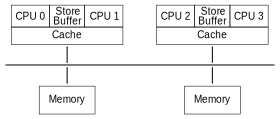
\includegraphics{memorder/NonMCAplatform}}
\caption{Shared Store Buffers And Multi-Copy Atomicity}
\label{fig:memorder:Shared Store Buffers And Multi-Copy Atomicity}
\end{figure}

This leads to the question of why a real system constrained by the
usual laws of physics would ever trigger the \co{exists} clause of
Listing~\ref{lst:memorder:WWC Litmus Test With Dependencies (No Ordering)}.
The cartoonish diagram of a such a real system is shown in
Figure~\ref{fig:memorder:Shared Store Buffers And Multi-Copy Atomicity}.
CPU~0 and CPU~1 share a store buffer, as do CPUs~2 and~3.
This means that CPU~1 can load a value out of the store buffer, thus
potentially immediately seeing a value stored by CPU~0.
In contrast, CPUs~2 and~3 will have to wait for the corresponding cache
line to carry this new value to them.

\QuickQuiz{}
	Then who would even \emph{think} of designing a system with shared
	store buffers???
\QuickQuizAnswer{
	This is in fact a very natural design for any system having
	multiple hardware threads per core.
	Natural from a hardware point of view, that is!
} \QuickQuizEnd

\begin{table*}
\small
\centering\OneColumnHSpace{-0.8in}
\begin{tabular}{r||l|l|l|l||l|l|l}
	& \tco{P0()} & \multicolumn{2}{c|}{\tco{P0()} \& \tco{P1()}} & \tco{P1()} & \multicolumn{3}{c}{\tco{P2()}} \\
	\cline{2-8}
	& Instruction & Store Buffer & Cache & Instruction &
			Instruction & Store Buffer & Cache \\
	\hline
	\hline
	1 & (Initial state) & & \tco{y==&b} &
		(Initial state) &
			(Initial state) & & \tco{x==&a} \\
	\hline
	2 & \tco{x = &x;} & \tco{x==&x} & \tco{y==&b} &
		 & & & \tco{x==&a} \\
	\hline
	3 & (Read-Invalidate \tco{x}) & \tco{x==&x} & \tco{y==&b} & \tco{r1 = x} (\tco{&x})
		 & & & \tco{x==&a} \\
	\hline
	4 &  & \tco{x==&x} \tco{y==&x} & \tco{y==&b} & \tco{y = r1}
		 & \tco{r2 = y} & & \tco{x==&a} \\
	\hline
	5 &  & \tco{x==&x} & \tco{y==&x} & (Finish store)
		 & (Read \tco{y}) & & \tco{x==&a} \\
	\hline
	6 & & \tco{x==&x} & \tco{y==&x} &
		 & (\tco{r2==&x}) & & \tco{x==&a} \tco{y==&x} \\
	\hline
	7 & & \tco{x==&x} & \tco{y==&x} &
		 & \tco{*r2 = &c} & \tco{y==&c} & \tco{x==&a} \tco{y==&x} \\
	\hline
	8 & & \tco{x==&x} & \tco{y==&x} &
		 & (Read Invalidate \tco{y}) & \tco{y==&c} & \tco{x==&a} \tco{y==&x} \\
	\hline
	9 & & \tco{x==&x} &  &
		 &  & \tco{y==&c} & \tco{x==&a} \tco{y==&x} \\
	\hline
	10 & & \tco{x==&x} &  &
		 & (Finish store) & & \tco{x==&a} \tco{y==&c} \\
	\hline
	11 & & \tco{x==&x} & \tco{x==&a} &
		 & (Respond \co{x}) & & \tco{y==&c} \\
	\hline
	12 & (Finish store) & & \tco{x==&x} &
		 &  & & \tco{y==&c} \\
\end{tabular}
\caption{Memory Ordering: WWC Sequence of Events}
\label{tab:memorder:Memory Ordering: WWC Sequence of Events}
\end{table*}

Table~\ref{tab:memorder:Memory Ordering: WWC Sequence of Events}
shows one sequence of events that can result in the \co{exists} clause in
Listing~\ref{lst:memorder:WWC Litmus Test With Dependencies (No Ordering)}
triggering.
This sequence of events will depend critically on \co{P0()} and
\co{P1()} sharing both cache and a store buffer in the manner shown in
Figure~\ref{fig:memorder:Shared Store Buffers And Multi-Copy Atomicity}.

\QuickQuiz{}
	But just how is it fair that P0 and P1 must share a store buffer
	and a cache, but P2 gets one each of its very own???
\QuickQuizAnswer{
	Presumably there is a P3, as is in fact shown in
	Figure~\ref{fig:memorder:Shared Store Buffers And Multi-Copy Atomicity},
	that shares P2's store buffer and cache.
	But not necessarily.
	Some platforms allow different cores to disable different numbers
	of threads, allowing the hardware to adjust to the needs of the
	workload at hand.
	For example, a single-threaded critical-path portion of the workload
	might be assigned to a core with only one thread enabled, thus
	allowing the single thread running that portion of the workload
	to use the entire capabilities of that core.
	Other more highly parallel but cache-miss-prone portions of the
	workload might be assigned to cores with all hardware threads
	enabled to provide improved throughput.
	This improved throughput could be due to the fact that while one
	hardware thread is stalled on a cache miss, the other hardware
	threads can make forward progress.

	In such cases, performance requirements override quaint human
	notions of fairness.
} \QuickQuizEnd

Row~1 shows the initial state, with the initial value of \co{y} in
P0's and P1's shared cache, and the initial value of \co{x} in
P2's cache.

Row~2 shows the immediate effect of \co{P0()} executing its write on line~13.
Because the cacheline containing \co{x} is not in \co{P0()}'s and \co{P1()}'s
shared cache, the new value (\co{&x})is stored in the shared store buffer.

Row~3 shows two transitions.
First, \co{P0()} issues a read-invalidate operation to fetch the cacheline
containing \co{x} so that it can flush the new value for \co{x} out of
the shared store buffer.
Second, \co{P1()} reads from \co{x} (line~20), an operation that completes
immediately because the new value of \co{x} is immediately available
from the shared store buffer.

Row~4 also shows two transitions.
First, it shows the immediate effect of \co{P1()} executing its write to
\co{y} (line~21), placing the new value into the shared store buffer.
Second, it shows the start of \co{P2()}'s read from \co{y} (line~28).

Row~5 continues the tradition of showing two transitions.
First, it shows \co{P1()} complete its store to \co{y}, flushing
from the shared store buffer to the cache.
Second, it shows \co{P2()} request the cacheline containing \co{x}.

Row~6 shows \co{P2()} receive the cacheline containing \co{y}, allowing
it to finish its load into \co{r2}, which takes on the value \co{&x}.

Row~7 shows \co{P2()} start executing its store to \co{y} (line~29), placing the
new value in is store buffer.

Row~8 shows \co{P2()} requesting exclusive ownership (``Read Invalidate'')
for the cacheline containing \co{y} in order to finish its store.

Row~9 shows the cacheline containing \co{y} removed from the shared cache,
so that \co{P2()} now has exclusive ownership.

Row~10 shows \co{P2()} completing its store to \co{y}, flushing the value
from its store buffer to its cache.

Row~11 shows \co{P2()} \emph{finally} responding to \co{P0()}'s request for
the cacheline containing \co{x}, which was made way back up on row~3.

Finally, row~12 shows \co{P0()} finish its store, flushing its value of
\co{x} from the shared store buffer to the shared cache.

Note well that the \co{exists} clause on line~32 has triggered.
The values of \co{r1} and \co{r2} are both the address of \co{x}, and
the final value of \co{x} is also the address of \co{x}.
This strange result occurred because \co{P0()}'s new value of \co{x} was
communicated to \co{P1()} long before it was communicated to \co{P2()}.

\QuickQuiz{}
	Referring to
	Table~\ref{tab:memorder:Memory Ordering: WWC Sequence of Events},
	why on earth would \co{P0()}'s store take so long to complete when
	\co{P1()}'s and \co{P2()}'s stores complete so quickly?
	In other words, does the \co{exists} clause on line~32 of
	Listing~\ref{lst:memorder:WWC Litmus Test With Dependencies (No Ordering)}
	really trigger on real systems?
\QuickQuizAnswer{
	You need to face the fact that it really can trigger.
	Akira Yokosawa used the \co{litmus7} tool to run this litmus test
	on a Power8 system.
	Out of 100,000,000,000 runs, 1,119 triggered the \co{exists}
	clause.
	Thus, triggering the \co{exists} clause is not merely a one-in-a-million
	occurrence, but rather a one-in-a-hundred-million occurrence.
	But it nevertheless really does trigger on real systems.
} \QuickQuizEnd

This counter-intuitive result happens because although dependencies
do provide ordering, they provide it only within the confines of their
own thread.
This three-thread example requires stronger ordering, which
is the subject of
Sections~\ref{sec:memorder:Cumulativity}
and~\ref{sec:memorder:Propagation}.

\subsubsection{Cumulativity}
\label{sec:memorder:Cumulativity}

\begin{figure*}[htbp]
\centering
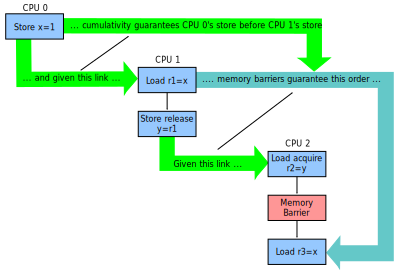
\includegraphics{memorder/memorybarriercum}
\caption{Cumulativity}
\label{fig:memorder:Cumulativity}
\end{figure*}

The three-thread example shown in
Listing~\ref{lst:memorder:WWC Litmus Test With Dependencies (No Ordering)}
requires \emph{cumulative} ordering, or \emph{cumulativity}.
As illustrated in
Figure~\ref{fig:memorder:Cumulativity}
given a cumulative ordering, any stores
from other threads whose values are returned by loads qualifying as
prior ordered operations will be seen as preceding any subsequent
ordered operations.

\begin{listing}[tbp]
{ \scriptsize
\begin{verbbox}[\LstLineNo]
C C-WWC+o+o-r+o-addr-o

{
int a = 0;
int b = 0;
int *c = &b;
int *x = &a;
int *y = &b;
}

P0(int **x)
{
  WRITE_ONCE(*x, x);
}

P1(int **x, int **y)
{
  int *r1;

  r1 = READ_ONCE(*x);
  smp_store_release(y, r1);
}

P2(int **y, int **c)
{
  int *r2;

  r2 = READ_ONCE(*y);
  WRITE_ONCE(*r2, c);
}

exists(1:r1=x /\ 2:r2=x /\ x=x)
\end{verbbox}
}
\centering
\theverbbox
\caption{WWC Litmus Test With Release}
\label{lst:memorder:WWC Litmus Test With Release}
\end{listing}

Dependencies do not provide cumulativity,
which is why the ``C'' column is blank for
both the \co{READ_ONCE()} and the \co{smp_read_barrier_depends()} rows
of Table~\ref{tab:memorder:Linux-Kernel Memory-Ordering Cheat Sheet}.
However, as indicated by the ``C'' in their ``C'' column,
release operations do provide cumulativity.
Therefore,
Listing~\ref{lst:memorder:WWC Litmus Test With Release}
substitutes a release operation for
Listing~\ref{lst:memorder:WWC Litmus Test With Dependencies (No Ordering)}'s
data dependency.
Because the release operation is cumulative, its ordering applies not only to
Listing~\ref{lst:memorder:WWC Litmus Test With Release}'s
load from \co{x} by \co{P1()} on line~20, but also to its store to \co{x}
by \co{P0()} on line~13---but only if that load returns the value stored,
which in this case is the address of \co{x}, which matches the \co{1:r1=x}
in the \co{exists} clause on line~32.
This means that \co{P2()}'s address dependency suffices to force the
write to \co{x} on line~29 to happen after the write on line~13, so
that the final value of \co{x} is the address of \co{c}, which
in turn prevents the \co{exists} clause from triggering.

In short, cumulativity can force non-multicopy-atomic platforms to
behave in a multi-copy-atomic manner in some situations.
Cumulativity nevertheless has limits, which are examined in the next section.

\subsubsection{Propagation}
\label{sec:memorder:Propagation}

% cumulativity not sufficient, sometimes also need propagation.

% @@@ write, release -> acquire, write -> read, smp_mb(), read

\subsubsection{Happens-Before}
\label{sec:memorder:Happens-Before}

% @@@ time as an implicit memory-ordering operation

@@@

Memory ordering and memory barriers can be extremely counter-intuitive.
For example, consider the functions shown in
Listing~\ref{lst:memorder:Parallel Hardware is Non-Causal}
executing in parallel
where variables~A, B, and~C are initially zero:

\begin{listing}[tbp]
{ \scriptsize
\begin{verbbox}
  1 thread0(void)
  2 {
  3   A = 1;
  4   smp_wmb();
  5   B = 1;
  6 }
  7
  8 thread1(void)
  9 {
 10   while (B != 1)
 11     continue;
 12   barrier();
 13   C = 1;
 14 }
 15
 16 thread2(void)
 17 {
 18   while (C != 1)
 19     continue;
 20   barrier();
 21   assert(A != 0);
 22 }
\end{verbbox}
}
\centering
\theverbbox
\caption{Parallel Hardware is Non-Causal}
\label{lst:memorder:Parallel Hardware is Non-Causal}
\end{listing}

Intuitively, \co{thread0()} assigns to~B after it assigns to~A,
\co{thread1()} waits until \co{thread0()} has assigned to~B before
assigning to~C, and \co{thread2()} waits until \co{thread1()} has
assigned to~C before referencing~A.
Therefore, again intuitively, the assertion on line~21 cannot possibly
fire.

This line of reasoning, intuitively obvious though it may be, is completely
and utterly incorrect.
Please note that this is \emph{not} a theoretical assertion:
actually running this code on real-world weakly-ordered hardware
(a 1.5\,GHz 16-CPU POWER 5 system) resulted in the assertion firing
16~times out of 10~million runs.
Clearly, anyone who produces code with explicit memory barriers
should do some extreme testing---although a proof of correctness might
be helpful, the strongly counter-intuitive nature of the behavior of
memory barriers should in turn strongly limit one's trust in such proofs.
The requirement for extreme testing should not be taken lightly, given
that a number of dirty hardware-dependent tricks were used to
greatly \emph{increase} the probability of failure in this run.

\QuickQuiz{}
	How on earth could the assertion on line~21 of the code in
	Listing~\ref{lst:memorder:Parallel Hardware is Non-Causal} on
	page~\pageref{lst:memorder:Parallel Hardware is Non-Causal}
	\emph{possibly} fail?
\QuickQuizAnswer{
	The key point is that the intuitive analysis missed is that
	there is nothing preventing the assignment to~C from overtaking
	the assignment to~A as both race to reach \co{thread2()}.
	This is explained in the remainder of this section.
} \QuickQuizEnd

\QuickQuiz{}
	Great \ldots So how do I fix it?
\QuickQuizAnswer{
	The easiest fix is to replace each of the \co{barrier()}s on
	line~12 and line~20 with an \co{smp_mb()}.

	Of course, some hardware is more forgiving than other hardware.
	For example, on x86 the assertion on line~21 of
	Listing~\ref{lst:memorder:Parallel Hardware is Non-Causal} on
	page~\pageref{lst:memorder:Parallel Hardware is Non-Causal}
	cannot trigger.
	On PowerPC, only the \co{barrier()} on line~20 need be
	replaced with \co{smp_mb()} to prevent the assertion from
	triggering.
} \QuickQuizEnd

So what should you do?
Your best strategy, if possible, is to use existing primitives that
incorporate any needed memory barriers, so that you can simply ignore
the rest of this chapter.

Of course, if you are implementing synchronization primitives,
you don't have this luxury.
The following discussion of memory ordering and memory barriers
is for you.

\section{What Can You Trust?}
\label{sec:memorder:What Can You Trust?}

You most definitely cannot trust your intuition.

What \emph{can} you trust?

It turns out that there are a few reasonably simple rules that
allow you to make good use of memory barriers.
This section derives those rules, for those who wish to get
to the bottom of the memory-barrier story, at least from the viewpoint
of portable code.
If you just want to be told what the rules are rather than suffering
through the actual derivation,
please feel free to skip to Section~\ref{sec:memorder:A Few Simple Rules}.

The exact semantics of memory barriers vary wildly from one CPU family to
another, so portable code must rely only on the least-common-denominator
semantics of memory barriers.

Fortunately, all CPU families impose the following rules:
\begin{enumerate}
\item	All accesses by a given CPU will appear to that CPU to have
	occurred in program order.
\item	All CPUs' accesses to a single variable will be consistent with
	some global ordering of stores to that variable.
\item	Memory barriers will operate in a pair-wise fashion.
\item	Operations will be provided from which exclusive locking
	primitives may be constructed.
\end{enumerate}

Therefore, if you need to use memory barriers in portable code,
you can rely on all of these properties.\footnote{
	Or, better yet, you can avoid explicit use of memory barriers
	entirely.
	But that would be the subject of other sections.}
Each of these properties is described in the following sections.

\subsection{Self-References Are Ordered}

A given CPU will see its own accesses as occurring in ``program order'',
as if the CPU was executing only one instruction at a time with no
reordering or speculation.
For older CPU families, this restriction is necessary for binary compatibility,
and only secondarily for the sanity of us software types.
There have been a few CPU families that violate this rule to a limited extent,
but in those cases, the compiler has been responsible
for ensuring that ordering is explicitly enforced as needed.

Either way, from the programmer's viewpoint, the CPU sees its own accesses
in program order.

\subsection{Single-Variable Memory Consistency}
\label{sec:memorder:Single-Variable Memory Consistency}

Because current commercially available computer systems provide
\emph{cache coherence},
if a group of CPUs all do concurrent non-atomic stores to a single variable,
the series of values seen by all CPUs will be consistent with at
least one global ordering.
For example, in the series of accesses shown in
Figure~\ref{fig:memorder:A Variable With Multiple Simultaneous Values},
CPU~1 sees the sequence {\tt \{1,2\}},
CPU~2 sees the sequence {\tt \{2\}},
CPU~3 sees the sequence {\tt \{3,2\}},
and
CPU~4 sees the sequence {\tt \{4,2\}}.
This is consistent with the global sequence {\tt \{3,1,4,2\}},
but also with all five of the other sequences of these four numbers that end
in~``2''.
Thus, there will be agreement on the sequence of values taken on
by a single variable, but there might be ambiguity.

In contrast, had the CPUs used atomic operations (such as the Linux kernel's
\co{atomic_inc_return()} primitive) rather than simple stores of
unique values, their observations would
be guaranteed to determine a single globally consistent sequence of values.
One of the \co{atomic_inc_return()} invocations would happen first,
and would change the value from~0 to~1, the second from~1 to~2, and
so on.
The CPUs could compare notes afterwards and come to agreement on the
exact ordering of the sequence of \co{atomic_inc_return()} invocations.
This does not work for the non-atomic stores described earlier because
the non-atomic stores do not return any indication of the earlier value,
hence the possibility of ambiguity.

Please note well that this section applies \emph{only} when all
CPUs' accesses are to one single variable.
In this single-variable case, cache coherence guarantees the
global ordering, at least assuming that some of the more aggressive
compiler optimizations are disabled via the Linux kernel's
\co{READ_ONCE()} and \co{WRITE_ONCE()} directives or C++11's relaxed
atomics~\cite{PeteBecker2011N3242}.
In contrast, if there are multiple variables, memory barriers are
required for the CPUs to consistently agree on the order for current
commercially available computer systems.

\section{Review of Locking Implementations}
\label{sec:memorder:Review of Locking Implementations}

\subsection{Semantics Sufficient to Implement Locking}

Suppose we have an exclusive lock (\co{spinlock_t} in the Linux
kernel, \co{pthread_mutex_t} in pthreads code) that guards a number
of variables (in other words, these variables are not accessed except
from the lock's critical sections).
The following properties must then hold true:
\begin{enumerate}
\item	A given CPU or thread must see all of its own loads and stores
	as if they had occurred in program order.
\item	The lock acquisitions and releases must appear to have executed
	in a single global order.\footnote{
		Of course, this order might be different from one run
		to the next.
		On any given run, however, all CPUs and threads must
		have a consistent view of the order of critical sections
		for a given exclusive lock.}
\item	Suppose a given variable has not yet been stored in a
	critical section that is currently executing.
	Then any load from a given variable performed in that critical section
	must see the last store to that variable from the last previous
	critical section that stored to it.
\end{enumerate}

The difference between the last two properties is a bit subtle:
the second requires that the lock acquisitions and releases occur
in a well-defined order, while the third requires that the critical
sections not ``bleed out'' far enough to cause difficulties for
other critical section.

Why are these properties necessary?

Suppose the first property did not hold.
Then the assertion in the following code might well fail!

\vspace{5pt}
\begin{minipage}[t]{\columnwidth}
\scriptsize
\begin{verbatim}
a = 1;
b = 1 + a;
assert(b == 2);
\end{verbatim}
\end{minipage}
\label{codesample:memorder:What Can You Count On? 1}
\vspace{5pt}

\QuickQuiz{}
	How could the assertion {\tt b==2} on
	page~\pageref{codesample:memorder:What Can You Count On? 1}
	possibly fail?
\QuickQuizAnswer{
	If the CPU is not required to see all of its loads and
	stores in order, then the {\tt b=1+a} might well see an
	old version of the variable~``a''.

	This is why it is so very important that each CPU or thread
	see all of its own loads and stores in program order.
} \QuickQuizEnd

Suppose that the second property did not hold.
Then the following code might leak memory!

\vspace{5pt}
\begin{minipage}[t]{\columnwidth}
\scriptsize
\begin{verbatim}
spin_lock(&mylock);
if (p == NULL)
  p = kmalloc(sizeof(*p), GFP_ATOMIC);
spin_unlock(&mylock);
\end{verbatim}
\end{minipage}
\label{codesample:memorder:What Can You Count On? 2}
\vspace{5pt}

\QuickQuiz{}
	How could the code on
	page~\pageref{codesample:memorder:What Can You Count On? 2}
	possibly leak memory?
\QuickQuizAnswer{
	Only the first execution of the critical section should
	see {\tt p==NULL}.
	However, if there is no global ordering of critical sections for
	{\tt mylock}, then how can you say that a particular one was
	first?
	If several different executions of that critical section thought
	that they were first, they would all see {\tt p==NULL}, and
	they would all allocate memory.
	All but one of those allocations would be leaked.

	This is why it is so very important that all the critical sections
	for a given exclusive lock appear to execute in some well-defined
	order.
} \QuickQuizEnd

Suppose that the third property did not hold.
Then the counter shown in the following code might well count backwards.
This third property is crucial, as it cannot be strictly true with
pairwise memory barriers.

\vspace{5pt}
\begin{minipage}[t]{\columnwidth}
\scriptsize
\begin{verbatim}
spin_lock(&mylock);
ctr = ctr + 1;
spin_unlock(&mylock);
\end{verbatim}
\end{minipage}
\label{codesample:memorder:What Can You Count On? 3}
\vspace{5pt}

\QuickQuiz{}
	How could the code on
	page~\pageref{codesample:memorder:What Can You Count On? 3}
	possibly count backwards?
\QuickQuizAnswer{
	Suppose that the counter started out with the value zero,
	and that three executions of the critical section had therefore
	brought its value to three.
	If the fourth execution of the critical section is not constrained
	to see the most recent store to this variable, it might well see
	the original value of zero, and therefore set the counter to
	one, which would be going backwards.

	This is why it is so very important that loads from a given variable
	in a given critical
	section see the last store from the last prior critical section to
	store to that variable.
} \QuickQuizEnd

If you are convinced that these rules are necessary, let's look at how
they interact with a typical locking implementation.

\subsection{Simple Locking Implementation}
\label{sec:memorder:Simple Locking Implementation}

Naive pseudocode for simple lock and unlock operations are shown below.
Note that the \co{atomic_xchg()} primitive implies a memory barrier
both before and after the atomic exchange operation, and that the
implicit barrier after the atomic exchange operation eliminates
the need for an explicit memory barrier in \co{spin_lock()}.
Note also that, despite the names, \co{atomic_read()} and
\co{atomic_set()} do \emph{not}
execute any atomic instructions, instead, it merely executes a
simple load and store, respectively.
This pseudocode follows a number of Linux implementations for
the unlock operation, which is a simple non-atomic store following a
memory barrier.
These minimal implementations must possess all the locking properties
laid out in Section~\ref{sec:memorder:What Can You Trust?}.

\vspace{5pt}
\begin{minipage}[t]{\columnwidth}
\scriptsize
\begin{verbatim}
  1 void spin_lock(spinlock_t *lck)
  2 {
  3   while (atomic_xchg(&lck->a, 1) != 0)
  4     while (atomic_read(&lck->a) != 0)
  5       continue;
  6 }
  7 
  8 void spin_unlock(spinlock_t lck)
  9 {
 10   smp_mb();
 11   atomic_set(&lck->a, 0);
 12 }
\end{verbatim}
\end{minipage}
\label{codesample:memorder:Naive Lock and Unlock Pseudocode}
\vspace{5pt}

The \co{spin_lock()} primitive cannot proceed until
the preceding \co{spin_unlock()} primitive completes.
If CPU~1 is releasing a lock that CPU~2 is attempting to acquire,
the sequence of operations might be as follows:

\vspace{5pt}
\begin{minipage}[t]{\columnwidth}
\tt \scriptsize
\begin{tabular}{l|l}
	\nf{CPU 1}		& \nf{CPU 2} \\
	\hline
	(critical section)	& \tco{atomic_xchg(&lck->a, 1)} $\rightarrow$1 \\
	<memory barrier>	& LOAD lck->a $\rightarrow$1 \\
	STORE lck->a = 0	& LOAD lck->a $\rightarrow$1 \\
				& LOAD lck->a $\rightarrow$0 \\
				& (implicit memory barrier \#1) \\
				& \tco{atomic_xchg(&lck->a, 1)} $\rightarrow$0 \\
				& (implicit memory barrier \#2) \\
				& (critical section) \\
\end{tabular}
\end{minipage}
\vspace{5pt}

In this particular case, pairwise memory barriers suffice to keep
the two critical sections in place.
CPU~2's \co{atomic_xchg(&lck->a, 1)} has seen CPU~1's \co{lck->a=0},
so therefore everything in CPU~2's following critical section must see
everything that CPU~1's preceding critical section did.
Conversely, CPU~1's critical section cannot see anything that CPU~2's
critical section will do.

\section{A Few Simple Rules}
\label{sec:memorder:A Few Simple Rules}

Probably the easiest way to understand memory barriers is to understand
a few simple rules:

\begin{enumerate}
\item	Each CPU sees its own accesses in order.
\item	If a single shared variable is loaded and stored by multiple
	CPUs, then the series of values seen by a given CPU will be
	consistent with the series seen by the other CPUs, and there
	will be at least one sequence consisting of all values stored
	to that variable with which each CPUs series will be
	consistent.\footnote{
		A given CPU's series may of course be incomplete,
		for example, if a given CPU never loaded or stored
		the shared variable, then it can have no opinion about
		that variable's value.}
\item	If one CPU does ordered stores to variables~A and~B,\footnote{
		For example, by executing the store to~A, a
		memory barrier, and then the store to~B.}
	and if a second CPU does ordered loads from~B and~A,\footnote{
		For example, by executing the load from~B, a
		memory barrier, and then the load from~A.}
	then if the second CPU's load from~B gives the value stored
	by the first CPU, then the second CPU's load from~A must
	give the value stored by the first CPU.
\item	If one CPU does a load from~A ordered before a store to~B,
	and if a second CPU does a load from~B ordered before a store to~A,
	and if the second CPU's load from~B gives the value stored by
	the first CPU, then the first CPU's load from~A must \emph{not}
	give the value stored by the second CPU.
\item	If one CPU does a load from~A ordered before a store to~B,
	and if a second CPU does a store to~B ordered before a
	store to~A, and if the first CPU's load from~A gives
	the value stored by the second CPU, then the first CPU's
	store to~B must happen after the second CPU's store to~B,
	hence the value stored by the first CPU persists.\footnote{
		Or, for the more competitively oriented, the first
		CPU's store to~B ``wins''.}
\end{enumerate}

\section{What Are Memory Barriers?}
\label{sec:memorder:What Are Memory Barriers?}

% @@@ rf, co, fr, and required strength.
% @@@ overview of memory barriers early, more details later.

As can be seen above, independent memory operations are effectively performed
in random order, but this can be a problem for CPU-CPU interaction and for I/O.
What is required is some way of intervening to instruct the compiler and the
CPU to restrict the order.

Memory barriers are such interventions.  They impose a perceived partial
ordering over the memory operations on either side of the barrier.

Such enforcement is important because the CPUs and other devices in a system
can use a variety of tricks to improve performance---including reordering,
deferral and combination of memory operations; speculative loads; speculative
branch prediction and various types of caching.  Memory barriers are used to
override or suppress these tricks, allowing the code to sanely control the
interaction of multiple CPUs and/or devices.

\subsection{Explicit Memory Barriers}
\label{sec:memorder:Explicit Memory Barriers}

Memory barriers come in four basic varieties:

\begin{enumerate}
\item	Write (or store) memory barriers,
\item	Data dependency barriers,
\item	Read (or load) memory barriers, and
\item	General memory barriers.
\end{enumerate}

Each variety is described below.

\subsubsection{Write Memory Barriers}

A write memory barrier gives a guarantee that all the STORE operations
specified before the barrier will appear to happen before all the STORE
operations specified after the barrier with respect to the other
components of the system.

A write barrier is a partial ordering on stores only; it is not required
to have any effect on loads.

A CPU can be viewed as committing a sequence of store operations to the
memory system as time progresses.  All stores before a write barrier will
occur in the sequence \emph{before} all the stores after the write barrier.

Note that write barriers should normally be paired with read
or data dependency barriers; see
% @@@ Section~\ref{sec:memorder:SMP Barrier Pairing}.

\subsubsection{Data Dependency Barriers}

A data dependency barrier is a weaker form of read barrier.  In the case
where two loads are performed such that the second depends on the result
of the first (e.g., the first load retrieves the address to which the second
load will be directed), a data dependency barrier would be required to
make sure that the target of the second load is updated before the address
obtained by the first load is accessed.

A data dependency barrier is a partial ordering on interdependent loads
only; it is not required to have any effect on stores, independent loads
or overlapping loads.

As mentioned for write memory barriers,
the other CPUs in the system can be viewed as
committing sequences of stores to the memory system that the CPU being
considered can then perceive.  A data dependency barrier issued by the CPU
under consideration guarantees that for any load preceding it, if that
load touches one of a sequence of stores from another CPU, then by the
time the barrier completes, the effects of all the stores prior to that
touched by the load will be perceptible to any loads issued after the data
dependency barrier.

See the @@@ % Section~\ref{sec:memorder:Examples of Memory Barrier Pairings} for
diagrams showing the ordering constraints.

Note that the first load really has to have a
\emph{data} dependency and
not a control dependency.  If the address for the second load is dependent
on the first load, but the dependency is through a conditional rather than
actually loading the address itself, then it's a \emph{control} dependency and
a full read barrier or better is required.  See
Section~\ref{sec:memorder:Control-Dependency Restrictions} for more information.

Note that data dependency barriers should normally be paired with
write barriers; see % @@@ Section~\ref{sec:memorder:SMP Barrier Pairing}.

\subsubsection{Read Memory Barriers}

A read barrier is a data dependency barrier plus a guarantee that all the
LOAD operations specified before the barrier will appear to happen before
all the LOAD operations specified after the barrier with respect to the
other components of the system.

A read barrier is a partial ordering on loads only; it is not required to
have any effect on stores.

Read memory barriers imply data dependency barriers, and so can substitute
for them.

Note that read barriers should normally be paired with write barriers;
see % @@@ Section~\ref{sec:memorder:SMP Barrier Pairing}.

\subsubsection{General Memory Barriers}

A general memory barrier gives a guarantee that all the LOAD and STORE
operations specified before the barrier will appear to happen before all
the LOAD and STORE operations specified after the barrier with respect to
the other components of the system.

A general memory barrier is a partial ordering over both loads and stores.

General memory barriers imply both read and write memory barriers, and so
can substitute for either.

\subsection{Implicit Memory Barriers}

There are a couple of types of implicit memory barriers, so called
because they are embedded into locking primitives:

\begin{enumerate}
\item	ACQUIRE operations and
\item	RELEASE operations.\footnote{
		Note that there were times when ACQUIRE/RELEASE operations
		were called as ``LOCK/UNLOCK'' operations in the Linux
		kernel community. ``ACQUIRE/RELEASE'' is preferred in
		discussing lockless techniques.}
\end{enumerate}

\subsubsection{ACQUIRE Operations}

An acuire operation acts as a one-way permeable barrier.
It guarantees that all memory
operations after the ACQUIRE operation will appear to happen after the ACQUIRE
operation with respect to the other components of the system.

Memory operations that occur before an ACQUIRE operation may appear to happen
after it completes.

An ACQUIRE operation should almost always be paired with a RELEASE operation.

\subsubsection{RELEASE Operations}

Release operations also act as a one-way permeable barrier.
It guarantees that all
memory operations before the RELEASE operation will appear to happen before
the RELEASE operation with respect to the other components of the system.

Memory operations that occur after a RELEASE operation may appear to
happen before it completes.

ACQUIRE and RELEASE operations are guaranteed to appear with respect to each
other strictly in the order specified.

The use of ACQUIRE and RELEASE operations generally precludes the need for
other sorts of memory barrier (but note the exceptions mentioned in the
@@@ % Section~\ref{sec:memorder:Device Operations}).

\QuickQuiz{}
	What effect does the following sequence have on the
	order of stores to variables~``a'' and~``b''?

	\vspace{5pt}
	\begin{minipage}[t]{\columnwidth}
	\small
	\begin{verbatim}
	STORE a = 1
	STORE b = 1
	<write barrier>
	\end{verbatim}
	\end{minipage}
\QuickQuizAnswer{
	Absolutely none.  This barrier {\em would} ensure that the
	assignments to~``a'' and~``b'' happened before any subsequent
	assignments, but it does nothing to enforce any order of
	assignments to~``a'' and~``b'' themselves.
} \QuickQuizEnd

\subsection{What May Not Be Assumed About Memory Barriers?}
\label{sec:memorder:What May Not Be Assumed About Memory Barriers?}

There are certain things that memory barriers cannot guarantee outside
of the confines of a given architecture:

\begin{enumerate}
\item	There is no guarantee that any of the memory accesses specified
	before a memory barrier will be \emph{complete} by the completion
	of a memory barrier instruction; the barrier can be considered
	to draw a line in that CPU's access queue that accesses of the
	appropriate type may not cross.
\item	There is no guarantee that issuing a memory barrier on one CPU
	will have any direct effect on another CPU or any other hardware
	in the system.	The indirect effect will be the order in which
	the second CPU sees the effects of the first CPU's accesses occur,
	but see the next point.
\item	There is no guarantee that a CPU will see the correct order
	of effects from a second CPU's accesses, even \emph{if} the second CPU
	uses a memory barrier, unless the first CPU \emph{also} uses a matching
	memory barrier (see
	% @@@ Section~\ref{sec:memorder:SMP Barrier Pairing}).
\item	There is no guarantee that some intervening piece of off-the-CPU
	hardware\footnote{
		This is of concern primarily in operating-system kernels.
		For more information on hardware operations and memory
		ordering, see the files \path{pci.txt}, \path{DMA-API-HOWTO.txt},
		and \path{DMA-API.txt} in the \path{Documentation} directory in
		the Linux source tree~\cite{Torvalds2.6kernel}.}
	will not reorder the memory accesses.  CPU cache
	coherency mechanisms should propagate the indirect effects of
	a memory barrier between CPUs, but might not do so in order.
\end{enumerate}

\subsection{Data Dependency Barriers (Again!)}
\label{sec:memorder:Data Dependency Barriers}

The usage requirements of data dependency barriers are a little subtle, and
it's not always obvious that they're needed.  To illustrate, consider the
following sequence of events (in pseudo asm), with initial values of shared
variables
{\tt \{A~=~1, B~=~2, C~=~3, P~=~\&A, Q~=~\&C\}}:

\vspace{5pt}
\begin{minipage}[t]{\columnwidth}
\tt
\scriptsize
\begin{tabular}{l|l}
	\nf{CPU 1}	& \nf{CPU 2} \\
	\hline
	STORE B = 4	& \\
	<write barrier>	& \\
	STORE P = \&B	& \\
			& Q = LOAD P \\
			& D = LOAD *Q \\
\end{tabular}
\end{minipage}
\vspace{5pt}

There's a clear data dependency here, and it would seem intuitively
obvious that by the end of the sequence, \co{Q}~must be either~\co{&A}
or~\co{&B}, and that:

\vspace{5pt}
\begin{minipage}[t]{\columnwidth}
\tt
\scriptsize
\begin{tabular}{c@{ implies }c}
	(Q == \&A) & (D == 1) \\
	(Q == \&B) & (D == 4) \\
\end{tabular}
\end{minipage}
\vspace{5pt}

Counter-intuitive though it might be, it is quite possible that
CPU~2's perception of~\co{P} might be updated \emph{before} its perception
of~\co{B}, thus leading to the following situation:

\vspace{5pt}
\begin{minipage}[t]{\columnwidth}
\tt
\scriptsize
\begin{tabular}{c@{ and }c}
	(Q == \&B) & (D == 2) ???? \\
\end{tabular}
\end{minipage}
\vspace{5pt}

Whilst this may seem like a failure of coherency or causality maintenance, it
isn't, and this behaviour can be observed on certain real CPUs (such as the DEC
Alpha).

To deal with this, a data dependency barrier must be inserted between the
address load and the data load (again with initial values of
{\tt \{A~=~1, B~=~2, C~=~3, P~=~\&A, Q~=~\&C\}}):

\vspace{5pt}
\begin{minipage}[t]{\columnwidth}
\tt
\scriptsize
\begin{tabular}{l|p{1.5in}}
	\nf{CPU 1}	& \nf{CPU 2} \\
	\hline
	STORE B = 4	& \\
	<write barrier>	& \\
	STORE P = \&B	& \\
			& Q = LOAD P \\
			& <data dependency barrier> \\
			& D = LOAD *Q \\
\end{tabular}
\end{minipage}
\vspace{5pt}

This enforces the occurrence of one of the two implications, and prevents the
third possibility from arising.

Note that this extremely counterintuitive situation arises most easily on
machines with split caches, so that, for example, one cache bank processes
even-numbered cache lines and the other bank processes odd-numbered cache
lines.
The pointer~\co{P} might be stored in an odd-numbered cache line, and the
variable~\co{B} might be stored in an even-numbered cache line.  Then, if the
even-numbered bank of the reading CPU's cache is extremely busy while the
odd-numbered bank is idle, one can see the new value of the
pointer~\co{P} (which is~\co{&B}),
but the old value of the variable~\co{B} (which is~2).

Another example of where data dependency barriers might by required is where a
number is read from memory and then used to calculate the index for an array
access with initial values
{\tt \{M[0]~=~1, M[1]~=~2, M[3]~=~3, P~=~0, Q~=~3\}}:

\vspace{5pt}
\begin{minipage}[t]{\columnwidth}
\tt
\scriptsize
\begin{tabular}{l|p{1.5in}}
	\nf{CPU 1} &	\nf{CPU 2} \\
	\hline
	M[1] = 4; & \\
	<write barrier> & \\
	P = 1;	&	\\
		&	Q = P; \\
		&	<data dependency barrier> \\
		&	D = M[Q]; \\
\end{tabular}
\end{minipage}
\vspace{5pt}

The data dependency barrier is very important to the Linux kernel's
RCU system, for example,
see \co{rcu_dereference()} in \path{include/linux/rcupdate.h}.
This permits the current
target of an RCU'd pointer to be replaced with a new modified target, without
the replacement target appearing to be incompletely initialized.

See also
Section~\ref{sec:memorder:Cache Coherency}
for a larger example.

% @@@ Section on READ_ONCE() and WRITE_ONCE()
% @@@ Convert some examples in "restrictions" sections to litmus tests

\subsection{Address- and Data-Dependency Restrictions}
\label{sec:memorder:Address- and Data-Dependency Restrictions}

Compilers do not understand either address or data dependencies,
although there are efforts underway to teach them, or at the very
least, standardize the process of teaching
them~\cite{PaulEMcKennneyConsumeP0190R0,PaulEMcKenney2017markconsumeP0462R1}.
In the meantime, it is necessary to be very careful in order to avoid
giving your compiler the opportunity to break your dependencies.

\subsubsection{Give your dependency chain a good start}
The load that heads your dependency chain must use proper
ordering, for example, \co{lockless_dereference()},
\co{rcu_dereference()}, or
a \co{READ_ONCE()} followed by \co{smp_read_barrier_depends()}.
Failure to follow this rule can have serious side effects:

\begin{enumerate}
\item	On DEC Alpha, a dependent load might not be ordered with
	the load heading the dependency chain, as described in
	Section~\ref{sec:app:whymb:Alpha}.
\item	If the load heading the dependency chain is a
	C11 non-volatile \co{memory_order_relaxed} load,
	the compiler could omit the load, for example, by using a value
	that it loaded in the past.
\item	If the load heading the dependency chain is a plain load,
	the compiler can omit the load, again by using a value
	that it loaded in the past.
	Worse yet, it could load twice instead of once, so that
	different parts of your code use different values---and
	real compilers do this, especially when under register
	pressure.
\item	The value loaded by the head of the dependency chain must
	be a pointer.
	In theory, yes, you could load an integer, perhaps to use
	it as an array index.
	In practice, the compiler knows too much about integers,
	and thus has way too many opportunities to break your
	dependency chain.
\end{enumerate}

\subsubsection{Avoid arithmetic dependency breakage}
Although it is just fine to do some arithmetic operations on a pointer in
your dependency chain, you need to be careful to avoid giving the
compiler too much information.
After all, if the compiler learns enough to determine the exact value
of the pointer, it can and sometimes will use that exact value instead
of the pointer itself.
As soon as the compiler does that, the dependency is broken and all
ordering is lost.

\begin{figure}[tbp]
{ \scriptsize
\begin{verbbox}
 1 int reserve_int;
 2 int *gp;
 3 int *p;
 4
 5 p = rcu_dereference(gp);
 6 if (p == &reserve_int)
 7   handle_reserve(p);
 8 do_something_with(*p); /* buggy! */
\end{verbbox}
}
\centering
\theverbbox
\caption{Breakable Dependencies With Comparisons}
\label{fig:memorder:Breakable Dependencies With Comparisons}
\end{figure}

\begin{figure}[tbp]
{ \scriptsize
\begin{verbbox}
 1 int reserve_int;
 2 int *gp;
 3 int *p;
 4
 5 p = rcu_dereference(gp);
 6 if (p == &reserve_int) {
 7   handle_reserve(&reserve_int);
 8   do_something_with(reserve_int); /* buggy! */
 9 } else {
10   do_something_with(*p); /* OK! */
11 }
\end{verbbox}
}
\centering
\theverbbox
\caption{Broken Dependencies With Comparisons}
\label{fig:memorder:Broken Dependencies With Comparisons}
\end{figure}

\begin{enumerate}
\item	Although it is permissible to compute offsets from a
	pointer, these offsets must not result in total cancellation.
	For example, given a \co{char} pointer \co{cp},
	\co{cp-(uintptr_t)cp)} will cancel and can allow the compiler
	to break your dependency chain.
	On the other hand, canceling offset values with each other
	is perfectly safe and legal.
	For example, if \co{a} and \co{b} are equal, \co{cp+a-b}
	is an identity function, including preserving the dependency.
\item	Comparisons can break dependencies.
	Figure~\ref{fig:memorder:Breakable Dependencies With Comparisons}
	shows how this can happen.
	Here global pointer \co{gp} points to a dynamically allocated
	integer, but if memory is low, it might instead point to
	the \co{reserve_int} variable.
	This \co{reserve_int} case might need special handling, as
	shown on lines~6 and~7 of the figure.
	But the compiler could reasonably transform this code into
	the form shown in
	Figure~\ref{fig:memorder:Broken Dependencies With Comparisons},
	especially on systems where instructions with absolute
	addresses run faster than instructions using addresses
	supplied in registers.
	However, there is clearly no ordering between the pointer
	load on line~5 and the dereference on line~8.
	Please note that this is simply an example: There are a great
	many other ways to break dependency chains with comparisons.
\end{enumerate}

\QuickQuiz{}
	Why can't you simply dereference the pointer before comparing it
	to \co{&reserve_int} on line~6 of
	Figure~\ref{fig:memorder:Breakable Dependencies With Comparisons}?
\QuickQuizAnswer{
	For first, it might be necessary to invoke
	\co{handle_reserve()} before \co{do_something_with()}.

	But more relevant to memory ordering, the compiler is often within
	its rights to hoist the comparison ahead of the dereferences,
	which would allow the compiler to use \co{&reserve_int} instead
	of the varaiable \co{p} that the hardware has tagged with
	a dependency.
} \QuickQuizEnd

\QuickQuiz{}
	But it should be safe to compare two pointer variables,
	right?  After all, the compiler doesn't know the value
	of either, so how can it possibly learn anything from the
	comparison?
\QuickQuizAnswer{

\begin{figure}[tbp]
{ \scriptsize
\begin{verbbox}
 1 int *gp1;
 2 int *gp2;
 3 int *p;
 4 int *q;
 5
 6 p = rcu_dereference(gp1);
 7 q = READ_ONCE(gp2);
 8 if (p == q)
 9   handle_equality(p);
10 do_something_with(*p);
\end{verbbox}
}
\centering
\theverbbox
\caption{Breakable Dependencies With Non-Constant Comparisons}
\label{fig:memorder:Breakable Dependencies With Non-Constant Comparisons}
\end{figure}

\begin{figure}[tbp]
{ \scriptsize
\begin{verbbox}
 1 int *gp1;
 2 int *gp2;
 3 int *p;
 4 int *q;
 5
 6 p = rcu_dereference(gp1);
 7 q = READ_ONCE(gp2);
 8 if (p == q) {
 9   handle_equality(q);
10   do_something_with(*q);
11 } else {
12   do_something_with(*p);
13 }
\end{verbbox}
}
\centering
\theverbbox
\caption{Broken Dependencies With Non-Constant Comparisons}
\label{fig:memorder:Broken Dependencies With Non-Constant Comparisons}
\end{figure}

	Unfortunately, the compiler really can learn enough to
	break your dependency chain, for example, as shown in
	Figure~\ref{fig:memorder:Breakable Dependencies With Non-Constant Comparisons}.
	The compiler is within its rights to transform this code
	into that shown in
	Figure~\ref{fig:memorder:Broken Dependencies With Non-Constant Comparisons},
	and might well make this transformation due to register pressure
	if \co{handle_equality()} was inlined and needed a lot of registers.
	Line~10 of this transformed code uses \co{q}, which although
	equal to \co{p}, is not necessarily tagged by the hardware as
	carrying a dependency.
	Therefore, this transformed code does not necessarily guarantee
	that line~10 is ordered after line~6.\footnote{
		Kudos to Linus Torvalds for providing this example.}
} \QuickQuizEnd

% @@@ Quick quiz showing other ways to break dependencies by comparison

\subsubsection{Safe comparison of dependent pointers}
It turns out that there are several safe ways to compare dependent
pointers:

\begin{enumerate}
\item	Comparisons against the \co{NULL} pointer.
	In this case, all the compiler can learn is that the pointer
	is \co{NULL}, in which case you are not allowed to
	dereference it in any case.
\item	The dependent pointer is never dereferenced, whether before or
	after the comparison.
\item	The dependent pointer is compared to a pointer that references
	objects that were last modified a very long time ago, where
	the safest value of ``a very long time ago'' is at compile time.
\end{enumerate}

@@@ convert to \co{uintptr_t} to set/clear bits and convert back.

% @@@ More here

\subsection{Control-Dependency Restrictions}
\label{sec:memorder:Control-Dependency Restrictions}

Control dependencies are especially tricky because current compilers
do not understand them and can easily break them.
The rules and examples in this section are intended to help you
prevent your compiler's ignorance from breaking your code.

A load-load control dependency requires a full read memory barrier,
not simply a data dependency barrier.
Consider the following bit of code:

\vspace{5pt}
\begin{minipage}[t]{\columnwidth}
\scriptsize
\begin{verbatim}
  1 q = READ_ONCE(x);
  2 if (q) {
  3   <data dependency barrier>
  4   q = READ_ONCE(y);
  5 }
\end{verbatim}
\end{minipage}
\vspace{5pt}

This will not have the desired effect because there is no actual data
dependency, but rather a control dependency that the CPU may short-circuit
by attempting to predict the outcome in advance, so that other CPUs see
the load from~\co{y} as having happened before the load from~\co{x}.
In such a case what's actually required is:

\vspace{5pt}
\begin{minipage}[t]{\columnwidth}
\scriptsize
\begin{verbatim}
  1 q = READ_ONCE(x);
  2 if (q) {
  3   <read barrier>
  4   q = READ_ONCE(y);
  5 }
\end{verbatim}
\end{minipage}
\vspace{5pt}

However, stores are not speculated.
This means that ordering \emph{is} provided for load-store control
dependencies, as in the following example:

\vspace{5pt}
\begin{minipage}[t]{\columnwidth}
\scriptsize
\begin{verbatim}
  1 q = READ_ONCE(x);
  2 if (q)
  3   WRITE_ONCE(y, 1);
\end{verbatim}
\end{minipage}
\vspace{5pt}

Control dependencies pair normally with other types of barriers.
That said, please note that neither \co{READ_ONCE()} nor \co{WRITE_ONCE()}
are optional!
Without the \co{READ_ONCE()}, the compiler might combine the load
from~\co{x} with other loads from~\co{x}.
Without the \co{WRITE_ONCE()}, the compiler might combine the store
to~\co{y} with other stores to~\co{y}.
Either can result in highly counterintuitive effects on ordering.

Worse yet, if the compiler is able to prove (say) that the value of
variable~\co{x} is always non-zero, it would be well within its rights
to optimize the original example by eliminating the ``\co{if}'' statement
as follows:

\vspace{5pt}
\begin{minipage}[t]{\columnwidth}
\scriptsize
\begin{verbatim}
  1 q = READ_ONCE(x);
  2 WRITE_ONCE(y, 1); /* BUG: CPU can reorder!!! */
\end{verbatim}
\end{minipage}
\vspace{5pt}

It is tempting to try to enforce ordering on identical stores on both
branches of the ``\co{if}'' statement as follows:

\vspace{5pt}
\begin{minipage}[t]{\columnwidth}
\scriptsize
\begin{verbatim}
 1 q = READ_ONCE(x);
 2 if (q) {
 3   barrier();
 4   WRITE_ONCE(y, 1);
 5   do_something();
 6 } else {
 7   barrier();
 8   WRITE_ONCE(y, 1);
 9   do_something_else();
10 }
\end{verbatim}
\end{minipage}
\vspace{5pt}

Unfortunately, current compilers will transform this as follows at high
optimization levels:

\vspace{5pt}
\begin{minipage}[t]{\columnwidth}
\scriptsize
\begin{verbatim}
 1 q = READ_ONCE(x);
 2 barrier();
 3 WRITE_ONCE(y, 1);  /* BUG: No ordering!!! */
 4 if (q) {
 5   do_something();
 6 } else {
 7   do_something_else();
 8 }
\end{verbatim}
\end{minipage}
\vspace{5pt}

Now there is no conditional between the load from~\co{x} and the store
to~\co{y}, which means that the CPU is within its rights to reorder them:
The conditional is absolutely required, and must be present in the
assembly code even after all compiler optimizations have been applied.
Therefore, if you need ordering in this example, you need explicit
memory barriers, for example, a release store:

\vspace{5pt}
\begin{minipage}[t]{\columnwidth}
\scriptsize
\begin{verbatim}
 1 q = READ_ONCE(x);
 2 if (q) {
 3   smp_store_release(&y, 1);
 4   do_something();
 5 } else {
 6   smp_store_release(&y, 1);
 7   do_something_else();
 8 }
\end{verbatim}
\end{minipage}
\vspace{5pt}

The initial \co{READ_ONCE()} is still required to prevent the compiler from
proving the value of~\co{x}.

In addition, you need to be careful what you do with the local variable~%
\co{q},
otherwise the compiler might be able to guess the value and again remove
the needed conditional.
For example:

\vspace{5pt}
\begin{minipage}[t]{\columnwidth}
\scriptsize
\begin{verbatim}
 1 q = READ_ONCE(x);
 2 if (q % MAX) {
 3   WRITE_ONCE(y, 1);
 4   do_something();
 5 } else {
 6   WRITE_ONCE(y, 2);
 7   do_something_else();
 8 }
\end{verbatim}
\end{minipage}
\vspace{5pt}

If \co{MAX} is defined to be~1, then the compiler knows that \co{(q\%MAX)} is
equal to zero, in which case the compiler is within its rights to
transform the above code into the following:

\vspace{5pt}
\begin{minipage}[t]{\columnwidth}
\scriptsize
\begin{verbatim}
 1 q = READ_ONCE(x);
 2 WRITE_ONCE(y, 2);
 3 do_something_else();
\end{verbatim}
\end{minipage}
\vspace{5pt}

Given this transformation, the CPU is not required to respect the ordering
between the load from variable~\co{x} and the store to variable~\co{y}.
It is tempting to add a \co{barrier()} to constrain the compiler,
but this does not help.
The conditional is gone, and the barrier won't bring it back.
Therefore, if you are relying on this ordering, you should make sure
that \co{MAX} is greater than one, perhaps as follows:

\vspace{5pt}
\begin{minipage}[t]{\columnwidth}
\scriptsize
\begin{verbatim}
 1 q = READ_ONCE(x);
 2 BUILD_BUG_ON(MAX <= 1);
 3 if (q % MAX) {
 4   WRITE_ONCE(y, 1);
 5   do_something();
 6 } else {
 7   WRITE_ONCE(y, 2);
 8   do_something_else();
 9 }
\end{verbatim}
\end{minipage}
\vspace{5pt}

Please note once again that the stores to~\co{y} differ.
If they were identical, as noted earlier, the compiler could pull this
store outside of the ``\co{if}'' statement.

You must also avoid excessive reliance on boolean short-circuit evaluation.
Consider this example:

\vspace{5pt}
\begin{minipage}[t]{\columnwidth}
\scriptsize
\begin{verbatim}
 1 q = READ_ONCE(x);
 2 if (q || 1 > 0)
 3   WRITE_ONCE(y, 1);
\end{verbatim}
\end{minipage}
\vspace{5pt}

Because the first condition cannot fault and the second condition is
always true, the compiler can transform this example as following,
defeating control dependency:

\vspace{5pt}
\begin{minipage}[t]{\columnwidth}
\scriptsize
\begin{verbatim}
 1 q = READ_ONCE(x);
 2 WRITE_ONCE(y, 1);
\end{verbatim}
\end{minipage}
\vspace{5pt}

This example underscores the need to ensure that the compiler cannot
out-guess your code.
More generally, although \co{READ_ONCE()} does force
the compiler to actually emit code for a given load, it does not force
the compiler to use the results.

In addition, control dependencies apply only to the then-clause and
else-clause of the if-statement in question.
In particular, it does
not necessarily apply to code following the if-statement:

\vspace{5pt}
\begin{minipage}[t]{\columnwidth}
\scriptsize
\begin{verbatim}
 1 q = READ_ONCE(x);
 2 if (q) {
 3   WRITE_ONCE(y, 1);
 4 } else {
 5   WRITE_ONCE(y, 2);
 6 }
 7 WRITE_ONCE(z, 1);  /* BUG: No ordering. */
\end{verbatim}
\end{minipage}
\vspace{5pt}

It is tempting to argue that there in fact is ordering because the
compiler cannot reorder volatile accesses and also cannot reorder
the writes to~\co{y} with the condition.
Unfortunately for this line
of reasoning, the compiler might compile the two writes to~\co{y} as
conditional-move instructions, as in this fanciful pseudo-assembly
language:

\vspace{5pt}
\begin{minipage}[t]{\columnwidth}
\scriptsize
\begin{verbatim}
 1 ld r1,x
 2 cmp r1,$0
 3 cmov,ne r4,$1
 4 cmov,eq r4,$2
 5 st r4,y
 6 st $1,z
\end{verbatim}
\end{minipage}
\vspace{5pt}

A weakly ordered CPU would have no dependency of any sort between the load
from~\co{x} and the store to~\co{z}.
The control dependencies would extend
only to the pair of cmov instructions and the store depending on them.
In short, control dependencies apply only to the stores in the ``\co{then}''
and ``\co{else}'' of the ``\co{if}'' in question (including functions
invoked by those two clauses), not to code following that ``\co{if}''.

Finally, control dependencies do \emph{not} provide cumulativity.\footnote{
	Refer to @@@ % Section~\ref{sec:memorder:Transitivity} for
	the meaning of transitivity.}
This is demonstrated by two related examples, with the initial values
of~\co{x} and~\co{y} both being zero:

\vspace{5pt}
\begin{minipage}[t]{\columnwidth}
\tt
\scriptsize
\begin{tabular}{l|p{1.5in}}
	\nf{CPU 0} &	\nf{CPU 1} \\
	\hline
	\tco{r1 = READ_ONCE(x);} &
		\tco{r2 = READ_ONCE(y);} \\
	if (r1 > 0) &
		if (r2 > 0) \\
	~~~\tco{WRITE_ONCE(y, 1);} &
		~~~\tco{WRITE_ONCE(x, 1);} \\
	\multicolumn{2}{l}{~} \\
	\multicolumn{2}{l}{\tco{assert(!(r1 == 1 && r2 == 1));}} \\
\end{tabular}
\end{minipage}
\vspace{5pt}

The above two-CPU example will never trigger the \co{assert()}.
However, if control dependencies guaranteed transitivity (which they do
not), then adding the following CPU would guarantee a related assertion:

\vspace{5pt}
\begin{minipage}[t]{\columnwidth}
\tt
\scriptsize
\begin{tabular}{l}
	\nf{CPU 2} \\
	\hline
	\tco{WRITE_ONCE(x, 2);} \\
	\multicolumn{1}{l}{~} \\
	\multicolumn{1}{l}{\tco{assert(!(r1 == 2 && r2 == 1 && x == 2));}} \\
\end{tabular}
\end{minipage}
\vspace{5pt}

But because control dependencies do \emph{not} provide transitivity, the above
assertion can fail after the combined three-CPU example completes.
If you need the three-CPU example to provide ordering, you will need
\co{smp_mb()} between the loads and stores in the CPU~0 and CPU~1 code
fragments, that is, just before or just after the ``\co{if}'' statements.
Furthermore, the original two-CPU example is very fragile and should be avoided.

The two-CPU example is known as LB (load buffering) and the three-CPU
example as WWC~\cite{Maranget2012TutorialARMPower}.

The following list of rules summarizes the lessons of this section:

\begin{enumerate}
\item	Compilers do not understand control dependencies, so it is
	your job to make sure that the compiler cannot break your code.

\item	Control dependencies can order prior loads against later stores.
	However, they do \emph{not} guarantee any other sort of ordering:
	Not prior loads against later loads, nor prior stores against
	later anything.
	If you need these other forms of ordering, use \co{smp_rmb()},
	\co{smp_wmb()}, or, in the case of prior stores and later loads,
	\co{smp_mb()}.

\item	If both legs of the ``\co{if}'' statement begin with identical stores
	to the same variable, then those stores must be ordered,
	either by preceding both of them with \co{smp_mb()} or by using
	\co{smp_store_release()} to carry out the stores.
	Please note that it is \emph{not} sufficient to use \co{barrier()}
	at beginning of each leg of the ``\co{if}'' statement because, as shown
	by the example above, optimizing compilers can destroy the control
	dependency while respecting the letter of the \co{barrier()} law.

\item	Control dependencies require at least one run-time conditional
	between the prior load and the subsequent store, and this
	conditional must involve the prior load.
	If the compiler is able to optimize the conditional away, it
	will have also optimized away the ordering.
	Careful use of \co{READ_ONCE()} and \co{WRITE_ONCE()} can help
	to preserve the needed conditional.

\item	Control dependencies require that the compiler avoid reordering
	the dependency into nonexistence.
	Careful use of \co{READ_ONCE()}, \co{atomic_read()}, or
	\co{atomic64_read()} can help to preserve your control
	dependency.

\item	Control dependencies apply only to the ``\co{then}'' and
	``\co{else}'' of the ``\co{if}'' containing the control
	dependency, including any functions that these two clauses call.
	Control dependencies do \emph{not} apply to code following the
	``\co{if}'' containing the control dependency.

\item	Control dependencies pair normally with other types of barriers.

\item	Control dependencies do \emph{not} provide transitivity.
	If you need transitivity, use \co{smp_mb()}.
\end{enumerate}

\subsection{Read Memory Barriers vs. Load Speculation}
\label{sec:memorder:Read Memory Barriers vs. Load Speculation}

Many CPUs speculate with loads: that is, they see that they will need to
load an item from memory, and they find a time where they're not using
the bus for any other loads, and then do the load in advance---even though
they haven't actually got to that point in the instruction execution
flow yet.
Later on, this potentially permits the actual load instruction to
complete immediately because the CPU already has the value on hand.

It may turn out that the CPU didn't actually need the value (perhaps because a
branch circumvented the load) in which case it can discard the value or just
cache it for later use.
For example, consider the following:

\vspace{5pt}
\begin{minipage}[t]{\columnwidth}
\tt
\scriptsize
\begin{tabular}{l|p{1.5in}}
	\nf{CPU 1} &	\nf{CPU 2} \\
	\hline
		&	LOAD B \\
		&	DIVIDE \\
		&	DIVIDE \\
		&	LOAD A \\
\end{tabular}
\end{minipage}
\vspace{5pt}

On some CPUs, divide instructions can take a long time to complete,
which means that CPU~2's bus might go idle during that time.
CPU~2 might therefore speculatively load~\co{A} before the divides
complete.
In the (hopefully) unlikely event of an exception from one of the dividees,
this speculative load will have been wasted, but in the (again, hopefully)
common case, overlapping the load with the divides will permit the load
to complete more quickly, as illustrated by
Figure~\ref{fig:memorder:Speculative Load}.

\begin{figure*}[htbp]
\centering
% \includegraphics{advsync-/SpeculativeLoad}
\caption{Speculative Load}
\ContributedBy{Figure}{fig:memorder:Speculative Load}{David Howells}
\end{figure*}

Placing a read barrier or a data dependency barrier just before the second
load:

\vspace{5pt}
\begin{minipage}[t]{\columnwidth}
\tt
\scriptsize
\begin{tabular}{l|p{1.5in}}
	\nf{CPU 1} &	\nf{CPU 2} \\
	\hline
		&	LOAD B \\
		&	DIVIDE \\
		&	DIVIDE \\
		&	<read barrier> \\
		&	LOAD A \\
\end{tabular}
\vspace{5pt}
\end{minipage}
%
will force any value speculatively obtained to be reconsidered to an extent
dependent on the type of barrier used.  If there was no change made to the
speculated memory location, then the speculated value will just be used,
as shown in
Figure~\ref{fig:memorder:Speculative Loads and Barrier}.
On the other hand, if there was an update or invalidation to~\co{A}
from some other CPU, then the speculation will be cancelled and the
value of~\co{A} will be reloaded,
as shown in Figure~\ref{fig:memorder:Speculative Loads Cancelled by Barrier}.

\begin{figure*}[htbp]
\centering
% \includegraphics{advsync-/SpeculativeLoadBarrier}
\caption{Speculative Load and Barrier}
\ContributedBy{Figure}{fig:memorder:Speculative Loads and Barrier}{David Howells}
\end{figure*}

\begin{figure*}[htbp]
\centering
% \includegraphics{advsync-/SpeculativeLoadBarrierCancel}
\caption{Speculative Load Cancelled by Barrier}
\ContributedBy{Figure}{fig:memorder:Speculative Loads Cancelled by Barrier}{David Howells}
\end{figure*}

\section{The Effects of the CPU Cache}
\label{sec:memorder:The Effects of the CPU Cache}

The perceived ordering of memory operations is affected by the caches
that lie between the CPUs and memory, as well as by the cache coherence
protocol that maintains memory consistency and ordering.
From a software viewpoint, these caches are for all intents and purposes
part of memory.
Memory barriers can be thought of as acting on the vertical dotted line in
Figure~\ref{fig:memorder:Memory Architecture}, ensuring that the CPU
presents its values to memory in the proper order, as well as ensuring
that it sees changes made by other CPUs in the proper order.

\begin{figure*}[htb]
\centering
% \includegraphics{advsync-/MemoryArchitecture}
\caption{Memory Architecture}
\ContributedBy{Figure}{fig:memorder:Memory Architecture}{David Howells}
\end{figure*}

Although the caches can ``hide'' a given CPU's memory accesses from the rest of
the system, the cache-coherence protocol ensures that all other CPUs see
any effects of these hidden accesses, migrating and invalidating cachelines
as required.
Furthermore, the CPU core may execute instructions in any order, restricted
only by the requirement that program causality and memory ordering
appear to be maintained.
Some of these instructions may generate memory accesses that must be queued
in the CPU's memory access queue, but execution may nonetheless continue
until the CPU either fills up its internal resources or until it must
wait for some queued memory access to complete.

\subsection{Cache Coherency}
\label{sec:memorder:Cache Coherency}

Although cache-coherence protocols guarantee that a given CPU sees its
own accesses in order, and that all CPUs agree on the order of modifications
to a single variable contained within a single cache line, there is no
guarantee that modifications to different variables will be seen in
the same order by all CPUs---although some computer systems do make
some such guarantees, portable software cannot rely on them.

\begin{figure*}[htb]
\centering
% \includegraphics{advsync-/SplitCache}
\caption{Split Caches}
\ContributedBy{Figure}{fig:memorder:Split Caches}{David Howells}
\end{figure*}

To see why reordering can occur, consider the two-CPU system shown in
Figure~\ref{fig:memorder:Split Caches}, in which each CPU has a split
cache.
This system has the following properties:
\begin{enumerate}
\item	An odd-numbered cache line may be in cache~A, cache~C,
	in memory, or some combination of the above.
\item	An even-numbered cache line may be in cache~B, cache~D,
	in memory, or some combination of the above.
\item	While the CPU core is interrogating one of its caches,\footnote{
		But note that in ``superscalar'' systems, the CPU
		might well be accessing both halves of its cache at
		once, and might in fact be performing multiple concurrent
		accesses to each of the halves.}
	its other cache is not necessarily quiescent.
	This other cache may instead be responding to an invalidation
	request, writing back a dirty cache line,
	processing elements in the CPU's memory-access queue, and
	so on.
\item	Each cache has queues of operations that need to be applied
	to that cache in order to maintain the required coherence
	and ordering properties.
\item	These queues are not necessarily flushed by loads from or
	stores to cache lines affected by entries in those queues.
\end{enumerate}

In short, if cache~A is busy, but cache~B is idle, then CPU~1's
stores to odd-numbered cache lines may be delayed compared to
CPU~2's stores to even-numbered cache lines.
In not-so-extreme cases, CPU~2 may see CPU~1's operations out
of order.

\IfInBook{Much more detail on memory ordering in hardware and software
	  may be found in Appendix~\ref{chp:app:whymb:Why Memory Barriers?}.
	 }
	 {}

\section{Where Are Memory Barriers Needed?}
\label{sec:memorder:Where Are Memory Barriers Needed?}

Memory barriers are only required where there's a possibility of interaction
between two CPUs or between a CPU and a device.  If it can be guaranteed that
there won't be any such interaction in any particular piece of code, then
memory barriers are unnecessary in that piece of code.

Note that these are the \emph{minimum} guarantees.
Different architectures may give
more substantial guarantees,
\IfInBook{as discussed in Appendix~\ref{chp:app:whymb:Why Memory Barriers?},}{}
but they may \emph{not}
be relied upon outside of code specifically designed to run only on
the corresponding architecture.

However, primitives that implement atomic operations, such as locking
primitives and atomic data-structure manipulation and traversal primitives,
will normally include any needed memory barriers in their definitions.
However, there are some exceptions, such as \co{atomic_inc()} in the
Linux kernel, so be sure to review the documentation, and, if possible,
the actual implementations, for your software environment.

One final word of advice: use of raw memory-barrier primitives should
be a last resort.
It is almost always better to use an existing primitive that takes
care of memory barriers.
